% Exact Affine Geometry, Central Radii, and Certified Compression Bounds
% for Finite-Outcome Quantum Instruments
\documentclass[11pt,a4paper]{article}

\usepackage[margin=2.5cm]{geometry}
\usepackage{amsmath,amssymb,amsthm}
\usepackage{mathtools}
\usepackage{booktabs}
\usepackage{tikz}
\usepackage{pgfplots}
\pgfplotsset{compat=1.18}
\usepackage[hidelinks]{hyperref}
\usepackage{enumitem}

\newtheorem{theorem}{Theorem}[section]
\newtheorem{lemma}[theorem]{Lemma}
\newtheorem{proposition}[theorem]{Proposition}
\newtheorem{corollary}[theorem]{Corollary}
\newtheorem{definition}[theorem]{Definition}
\newtheorem{remark}[theorem]{Remark}
\newtheorem{convention}[theorem]{Convention}
\newtheorem{example}[theorem]{Example}

\newcommand{\Lin}{\mathrm{L}}
\newcommand{\Herm}{\mathrm{Herm}}
\newcommand{\Sstate}{\mathcal{S}}
\newcommand{\Chan}{\mathrm{Chan}}
\newcommand{\Inst}{\mathrm{Inst}}
\newcommand{\RepInst}{\mathrm{RepInst}}
\newcommand{\Tr}{\operatorname{Tr}}
\newcommand{\id}{\operatorname{id}}
\newcommand{\supp}{\operatorname{supp}}
\newcommand{\rank}{\operatorname{rank}}
\newcommand{\diam}{\operatorname{diam}}
\newcommand{\coind}{\operatorname{coind}_{\mathbb Z_2}}
\newcommand{\Jhat}{\widehat J}
\newcommand{\vD}{\vec{\Delta}}
\newcommand{\aff}{\operatorname{aff}}

\title{\bf Exact Affine Geometry, Optimal Centres, and Certified Compression Bounds for Finite-Outcome Quantum Instruments}
\author{Anonymous}
\date{}

\begin{document}
\maketitle

\begin{abstract}
Quantum instruments describe the full statistics of a measurement together with the conditional post-measurement state, and they form the building blocks of adaptive protocols and quantum networks. We study the geometry of the set of all $n$-outcome instruments acting between two finite-dimensional quantum systems, and we ask how many continuous latent parameters are needed to encode an arbitrary instrument and later reconstruct it with uniformly small error, under the convention of continuous encoding and unrestricted decoding. The geometry of the instrument body is determined exactly: its affine dimension is $d_A^2(nd_B^2-1)$; the largest diamond-norm ball contained in the body has radius $2/(nd_B\min\{d_A,d_B\})$ and is centred at the uniform depolarising instrument, which is optimal among all centres; and the same instrument is optimal for the covering problem, with an exact covering radius linked to the in-radius by a complementarity identity. Every radius and width carries a single-shot operational meaning through the optimal discrimination error. On the compression side, antipodal constructions --- output preparation, an input-dependent observable sphere, and a full-direction section --- produce a certified lower envelope on the optimal error, matched by constructive upper bounds from constant codes, convex projection, and balanced pinching; the zero-error threshold equals the affine dimension. The single-outcome case recovers quantum channels, treated in a companion paper, and the one-dimensional-output case recovers finite-outcome measurements; the trade-off between the number of outcomes and the robustness of the uniform instrument is made explicit.
\end{abstract}

\noindent\textbf{Keywords:} quantum instruments; diamond norm; compression width; antipodal profile; Chebyshev radius; quantum measurements; no-programming theorem.


\tableofcontents

\section{Introduction}
\label{sec:intro}

Quantum instruments are the natural generalisation of quantum channels to finite-outcome statistics: a collection of completely positive, trace-nonincreasing maps whose sum is a channel. They describe both the probability of an outcome and the conditional post-measurement state, and they model finite-outcome measurements, adaptive protocols, and the nodes of quantum networks~\cite{DaviesLewis1970,Ozawa1984,ChiribellaEtAl2009Instruments,ChiribellaEtAl2008Combs}.

The general source--latent theory underlying the obstruction arguments --- fiber radii, antipodal profiles, deleted-product coindex, and stable Lipschitz variants --- is developed in the companion paper~\cite{CompanionChannels}, which treats the channel case; the present paper uses the specialisations recorded in Section~\ref{sec:prelim}. Throughout, the $n=1$ restrictions of the instrument theorems below recover the corresponding channel-level statements of~\cite{CompanionChannels}: the observable sphere, the full-direction sphere, the join, the global in-radius, and the covering results.

The question treated here is the instrument-level analogue of the channel problem: does the compact convex body of $n$-outcome instruments between $A$ and $B$ admit a continuous low-dimensional latent encoding with uniformly accurate decoding? Throughout, we adopt the standard asymmetric convention: the \emph{encoder is continuous} and the \emph{decoder is unrestricted} (Convention~\ref{conv:decoder}); where a continuous decoder is additionally available we say so explicitly. The answer has three regimes. At small latent dimension, input-independent preparation of a flagged output state already forces error one. In an intermediate range, the width is bracketed between a certified lower and a certified upper envelope: a centred-ball bound scaling as $1/n$ --- which Theorem~\ref{thm:global-inradius} shows is the best centred-ball certificate at any centre --- plus a full-direction antipodal obstruction contributing an $n$-independent component $1/d_A$, against upper bounds that never sink below one. From the affine dimension on, exact reconstruction holds, even with a continuous decoder.

The main contribution of this paper is the exact affine geometry of the instrument body and its compression consequences: the affine dimension, the centred and global in-radii, the covering radius, and the diameter are determined exactly, with the uniform depolarising instrument turning out to be an optimal centre simultaneously for the in-radius and the covering radius (a concave--convex duality, Theorem~\ref{thm:global-inradius} and Remark~\ref{rem:duality}). Which quantities are determined \emph{exactly}, and which only by \emph{certified bounds}, is stated once in Remark~\ref{rem:exact-vs-certified} and maintained throughout. A separate physical question --- whether an abstract code can be realised by a fixed programmable processor --- is addressed in Appendix~\ref{app:no-programming}: exact finite-dimensional evaluation of all unitary channels is impossible, and vanishing error forces unbounded program dimension. This separates \emph{representational} dimension from \emph{programmable} evaluation; the main theorems do not rely on the appendix.

The paper is organised as follows. Section~\ref{sec:prelim} fixes notation and records the specialised forms of the companion source--latent theory used throughout. Section~\ref{sec:exact-geometry} determines the exact affine and metric parameters of the instrument body, and Section~\ref{sec:lower} constructs the antipodal certificates and the certified lower envelope. Section~\ref{sec:widths} develops the constructive upper bounds and the exact thresholds, and Section~\ref{sec:specialisations} collects the specialisations, worked examples, and the outcome trade-off. Section~\ref{sec:conclusion} summarises which quantities are exact and which are certified and lists the open problems; Appendix~\ref{app:no-programming} records the no-programming background.

\section{Preliminaries}
\label{sec:prelim}

Throughout, $A$ and $B$ are finite-dimensional Hilbert spaces of dimensions $d_A,d_B$, and $n\in\mathbb N$ is the number of outcomes. Let $A_0\simeq A$ be a reference copy with a fixed pair of conjugate bases in $A_0$ and $A$, and define the maximally entangled state
\[
|\omega_A\rangle=\frac1{\sqrt{d_A}}\sum_{j=1}^{d_A}|j\rangle_{A_0}|j\rangle_A.
\]
For a map $\Phi:\Lin(A)\to\Lin(B)$ the \emph{normalised Choi operator} is
\[
\Jhat_\Phi=(\id_{A_0}\otimes\Phi)(|\omega_A\rangle\langle\omega_A|),
\]
the Choi--Jamio{\l}kowski isomorphism in the normalised form~\cite{Choi1975,Jamiolkowski1972}.

\begin{remark}[Normalised Choi convention]
\label{rem:choi-convention}
With the unnormalised maximally entangled vector $|\Omega_A\rangle=\sum_j|j\rangle_{A_0}|j\rangle_A$ one has $\Jhat_\Phi=\tfrac1{d_A}J_\Phi^{\mathrm{unnorm}}$. Consequently $\Phi$ is trace preserving if and only if
\[
\Tr_B\Jhat_\Phi=\frac{I_{A_0}}{d_A}.
\]
All affine constraints, radii, covering bounds, and pinching dimension counts in this paper use this normalised convention.
\end{remark}

Let $C_n$ be an $n$-dimensional classical flag space with basis $|1\rangle,\dots,|n\rangle$.

\begin{definition}[Instrument, flagged channel, and instrument diamond norm]
An $n$-outcome instrument from $A$ to $B$ is a tuple $\mathcal I=(\mathcal I_1,\dots,\mathcal I_n)$ of completely positive, trace-nonincreasing maps whose sum is a channel. Write $\Inst_n(A,B)$ for the set of all such instruments. The flagged channel of $\mathcal I$ is
\[
\widehat{\mathcal I}(X)=\sum_{k=1}^n\mathcal I_k(X)\otimes|k\rangle\langle k|.
\]
For a tuple $\vD=(\Delta_1,\dots,\Delta_n)$ of Hermiticity-preserving maps, define the flagged map and the instrument diamond norm by
\[
\widehat{\vD}(X)=\sum_{k=1}^n\Delta_k(X)\otimes|k\rangle\langle k|,
\qquad
\|\vD\|_{\diamond,\mathrm{inst}}=\|\widehat{\vD}\|_\diamond.
\]
By block diagonality (the trace norm of a block-diagonal operator is the sum of the trace norms of its blocks) this equals the operational formula
\[
\|\vD\|_{\diamond,\mathrm{inst}}
=\sup_{\rho\in\Sstate(A_0\otimes A)}
\sum_{k=1}^n\|(\id_{A_0}\otimes\Delta_k)(\rho)\|_1.
\]
The diamond norm was introduced in~\cite{AharonovKitaevNisan1998}; a reference system of input dimension $d_A$ suffices for it~\cite{Watrous2018}. The summands are the unconditional, generally subnormalised outcome contributions. The body $\Inst_n(A,B)$ is compact and convex: convexity follows from the convexity of the completely positive cone and the affine normalisation constraints, and compactness from positivity together with the summed marginal condition, which bounds every Choi block.
\end{definition}

\begin{remark}[Operational meaning]
\label{rem:operational}
For two instruments $\mathcal I,\mathcal J$ with equal prior probabilities, the optimal single-use discrimination success probability, with arbitrary reference assistance, is
\[
p_{\mathrm{succ}}
=\frac12+\frac14\,\|\mathcal I-\mathcal J\|_{\diamond,\mathrm{inst}},
\]
i.e.\ the advantage over random guessing is $\tfrac14\|\mathcal I-\mathcal J\|_{\diamond,\mathrm{inst}}$ (an instance of the Holevo--Helstrom theorem for binary state discrimination~\cite{Helstrom1976}, applied to the flagged outputs). Thus every radius and width stated in the instrument diamond norm has a direct single-shot discrimination interpretation, up to this conventional factor of $1/4$.
\end{remark}

The ambient affine space and its direction space are
\begin{align*}
\mathfrak A_{A,B}^{(n)}
&=\Big\{(\Phi_1,\dots,\Phi_n):
\Phi_k\ \text{Hermiticity-preserving},\quad
\sum_{k=1}^n\Tr_B\Jhat_{\Phi_k}=\frac{I_{A_0}}{d_A}\Big\},\\
\mathfrak V_{A,B}^{(n)}
&=\Big\{(\Delta_1,\dots,\Delta_n):
\Delta_k\ \text{Hermiticity-preserving},\quad
\sum_{k=1}^n\Tr_B\Jhat_{\Delta_k}=0\Big\}.
\end{align*}
Here $\mathfrak V_{A,B}^{(n)}$ is the real linear direction space, of real dimension $D_{A,B}^{(n)}$ when $nd_B>1$.
Thus only the summed direction is trace-annihilating; individual outcome components need not be. For $\mathcal I_0\in\mathfrak A_{A,B}^{(n)}$ define the closed relative instrument-diamond ball
\[
\overline B_{\diamond,\mathrm{inst}}^{\mathrm{rel}}(\mathcal I_0,\rho)
=\big\{\mathcal I_0+\vD:\vD\in\mathfrak V_{A,B}^{(n)},\ \|\vD\|_{\diamond,\mathrm{inst}}\le\rho\big\},
\]
and, for $\mathcal I_0\in\Inst_n(A,B)$, its centred relative in-radius
\[
\rho_{\diamond,\mathrm{inst}}(\mathcal I_0)
=\sup\Big\{\rho\ge0:
\overline B_{\diamond,\mathrm{inst}}^{\mathrm{rel}}(\mathcal I_0,\rho)
\subseteq\Inst_n(A,B)\Big\}.
\]
Let $\mathcal I_*$ be the uniform depolarising instrument, $(\mathcal I_*)_k=\Omega_{A,B}/n$, where $\Omega_{A,B}(X)=\Tr(X)I_B/d_B$, so that $\Jhat_{(\mathcal I_*)_k}=I_{A_0\otimes B}/(n d_Ad_B)$.

\begin{remark}[POVM case $d_B=1$]
\label{rem:povm}
When $d_B=1$, identify $\Lin(B)$ with $\mathbb C$. An instrument component is a positive functional $\mathcal I_k(X)=\Tr(E_kX)$ for a unique effect $E_k\ge0$, and the instrument condition is exactly $\sum_{k=1}^nE_k=I_A$. Thus $\Inst_n(A,\mathbb C)$ is the convex body of $n$-outcome POVMs on $A$.
\end{remark}

\begin{remark}[Degenerate singleton case]
\label{rem:degenerate}
If $n=d_B=1$, then $\Inst_1(A,\mathbb C)$ consists of the unique trace functional $X\mapsto\Tr(X)$: its affine dimension is $D_{A,1}^{(1)}=0$, its direction space is $\{0\}$, every compression width is $0$, and, because every relative ball is the singleton, the centred relative in-radius is $+\infty$ under the supremum convention. Except where explicitly stated, all nontrivial statements in this paper assume
\[
n d_B>1.
\]
\end{remark}

\begin{remark}[Exact claims versus certified bounds]
\label{rem:exact-vs-certified}
The following statements are exact: (i) the affine dimension $D_{A,B}^{(n)}$; (ii) the centred in-radius at the uniform instrument; (iii) the global in-radius over all centres, which equals (ii) by Theorem~\ref{thm:global-inradius}; (iv) the global covering radius and optimality of $\mathcal I_*$ as a centre; (v) the diameter, equal to $2$; (vi) the antipodal profile of the replacement body, and hence of the full body when $d_A=1$; (vii) the constant-code width $\delta_{0,\mathrm{inst}}^{\diamond}(A,B)=R_{\mathrm{inst}}(\mathcal I_*)$; (viii) the zero-error Euclidean threshold for continuous encoding with unrestricted decoding; (ix) the full width function in the collapse case $nd_Bs=2$ (Theorem~\ref{thm:collapse}). The following are certified bounds or open quantities, not exact determinations: (a) the intermediate compression widths $\delta_{r,\mathrm{inst}}^{\diamond}(A,B)$ for $0<r<D_{A,B}^{(n)}$; (b) the full antipodal profile beyond the certified constructions; (c) optimality of the certified upper envelope $U_r^{(n)}$. Table~\ref{tab:summary} collects the complete regime-by-regime picture.
\end{remark}

\begin{remark}[Notation]
\label{rem:notation}
To avoid collisions, the following symbols are used consistently: ranks are denoted $r_E$, the number of input pinching blocks by $k_{\mathrm{in}}$, the number of output pinching blocks by $\ell_{\mathrm{out}}$, the latent dimension by $r$ (or $q$ for general latent spaces), the covering radius by $R$, input or support subspaces by $W$, and the reference system in the covering arguments by $E$.
\end{remark}

\section{Exact affine and metric parameters}
\label{sec:exact-geometry}

This section determines the affine dimension, the centred in-radius at the uniform instrument, the global in-radius, the covering radius, and the diameter of the instrument body, all exactly.

\begin{proposition}[Affine dimension of the instrument body]
\label{prop:dimension}
Assume $nd_B>1$. Then
\[
\dim_{\mathbb R}\aff\,\Inst_n(A,B)
=D_{A,B}^{(n)}:=d_A^2(nd_B^2-1).
\]
\end{proposition}

\begin{proof}
An instrument Choi tuple consists of $n$ Hermitian operators on $A_0\otimes B$, of total real dimension $nd_A^2d_B^2$. The normalisation constraint
\[
\sum_{k=1}^n\Tr_B\Jhat_{\mathcal I_k}=\frac{I_{A_0}}{d_A}
\]
imposes $d_A^2=\dim_{\mathbb R}\Herm(A_0)$ real affine equations. The linear map $(X_1,\dots,X_n)\mapsto\sum_k\Tr_BX_k$ from $\bigoplus_k\Herm(A_0\otimes B)$ to $\Herm(A_0)$ is surjective: for $H\in\Herm(A_0)$ set $X_1=H\otimes I_B/d_B$ (so $\Tr_BX_1=H$) and $X_{k\ge2}=0$. Hence the constraints are independent. The tuple of $\mathcal I_*$ has every block $\Jhat_{(\mathcal I_*)_k}=I_{A_0\otimes B}/(nd_Ad_B)$ \emph{positive definite}; every sufficiently small Hermitian perturbation in $\mathfrak V_{A,B}^{(n)}$ therefore remains positive semidefinite. Hence $\mathcal I_*$ is a relative interior point, positivity introduces no further affine equalities, and the affine count $nd_A^2d_B^2-d_A^2=d_A^2(nd_B^2-1)$ is attained.
\end{proof}

\begin{lemma}[Instrument spectral bound]
\label{lem:spectral}
Let $s=\min\{d_A,d_B\}$ and $\vD\in\mathfrak V_{A,B}^{(n)}$. Let
\[
X=\Jhat_{\widehat{\vD}}\in\Herm(A_0\otimes B\otimes C_n),\qquad
X=\sum_{k=1}^nX_k\otimes|k\rangle\langle k|,\quad X_k=\Jhat_{\Delta_k},
\]
be the normalised Choi operator of the flagged map $\widehat{\vD}:A\to B\otimes C_n$. Then
\[
\max\{0,\lambda_{\max}(-X)\}\le\frac{s}{2d_A}\|\vD\|_{\diamond,\mathrm{inst}}.
\]
\end{lemma}

\begin{proof}
If $\lambda_{\max}(-X)\le0$ there is nothing to prove. Otherwise, since $X$ is block diagonal, $\lambda_{\max}(-X)=\max_k\lambda_{\max}(-X_k)$. Choose $k_0$ attaining the maximum and a unit vector $|v\rangle\in A_0\otimes B$ with $X_{k_0}|v\rangle=-\lambda|v\rangle$, $\lambda=\lambda_{\max}(-X)$. Write $W\subseteq A_0$ for the support of the $B$-marginal $\Tr_B|v\rangle\langle v|$ and set $b=\dim W$; the marginal of a pure state has rank equal to its Schmidt rank, so $b\le s=\min\{d_A,d_B\}$. If $|e_1\rangle,\dots,|e_b\rangle$ is an orthonormal basis of $W$ and $|\overline e_j\rangle\in A$ its coordinatewise conjugate under the fixed Choi bases, define
\[
|\omega_W\rangle=\frac1{\sqrt b}\sum_{j=1}^b|e_j\rangle_{A_0}|\overline e_j\rangle_A.
\]
With $P_W$ the projection onto $W$, the normalised-Choi convention gives
\[
Y:=(\id_{A_0}\otimes\widehat{\vD})(|\omega_W\rangle\langle\omega_W|)
=\frac{d_A}{b}(P_W\otimes I_{B\otimes C_n})X(P_W\otimes I_{B\otimes C_n}).
\]
The direction constraint implies
\[
\Tr Y=\frac{d_A}{b}\Tr\Big[P_W\sum_{k=1}^n\Tr_BX_k\Big]=0,
\]
so $Y$ is Hermitian and traceless. Since $|v\rangle\in W\otimes B$, testing on $|v,k_0\rangle:=|v\rangle\otimes|k_0\rangle$ gives
\[
\langle v,k_0|Y|v,k_0\rangle=-\frac{d_A}{b}\lambda.
\]
A traceless Hermitian operator $Y=Y_+-Y_-$ satisfies $\Tr Y_+=\Tr Y_-=\tfrac12\|Y\|_1$, and for every unit vector $|w\rangle$ one has $\langle w|Y|w\rangle\ge-\Tr Y_-$: indeed $Y\ge-Y_-$ implies $\langle w|Y|w\rangle\ge-\langle w|Y_-|w\rangle\ge-\Tr Y_-$. Consequently
\[
\|Y\|_1\ge-2\langle v,k_0|Y|v,k_0\rangle
=\frac{2d_A}{b}\lambda\ge\frac{2d_A}{s}\lambda.
\]
The state $|\omega_W\rangle\langle\omega_W|$ is admissible in the instrument diamond-norm optimisation, so $\|\vD\|_{\diamond,\mathrm{inst}}\ge\|Y\|_1$, and rearranging proves the claim. The entangled input thus plays two roles at once: its Schmidt support $W$ selects the subspace on which the negative eigenvalue of the perturbation is read out, the normalised-Choi convention amplifying it by the factor $d_A/b$; and the same state is an admissible reference-assisted input, so the resulting trace-norm bound on $Y$ is automatically a lower bound in the instrument diamond norm. This double role is the reason the input dimension appears in the denominator of the spectral bound: a perturbation can distribute its negativity across all $d_A$ Choi coordinates, while the entangled input concentrates it back onto the $b$-dimensional Schmidt support of the witness, amplifying the negative eigenvalue by the factor $d_A/b$.
\end{proof}

\begin{theorem}[Instrument diamond ball]
\label{thm:ball}
Let $s=\min\{d_A,d_B\}$. Then
\[
\overline B_{\diamond,\mathrm{inst}}^{\mathrm{rel}}\Big(\mathcal I_*,\frac{2}{nd_Bs}\Big)
\subseteq\Inst_n(A,B).
\]
\end{theorem}

\begin{proof}
Every eigenvalue of the flagged Choi operator of $\mathcal I_*$ equals $1/(nd_Ad_B)$. If $\vD\in\mathfrak V_{A,B}^{(n)}$ with $\|\vD\|_{\diamond,\mathrm{inst}}\le2/(nd_Bs)$ and $X=\Jhat_{\widehat{\vD}}$, Lemma~\ref{lem:spectral} gives
\[
\lambda_{\max}(-X)\le\frac{s}{2d_A}\cdot\frac{2}{nd_Bs}=\frac1{nd_Ad_B}=\lambda_{\min}(\Jhat_{\mathcal I_*}),
\]
so the full flagged Choi operator $\Jhat_{\mathcal I_*}+X$ is positive. Since $X$ is block diagonal this is equivalent to positivity of every outcome block, so each perturbed component is completely positive. The summed marginal is unchanged by the direction constraint, so the sum is trace preserving; and because the blocks are positive with $\sum_k\Tr_B(\Jhat_{(\mathcal I_*)_k}+X_k)=I_{A_0}/d_A$, each partial trace is bounded by $I_{A_0}/d_A$, so each component is trace-nonincreasing. Hence $\mathcal I_*+\vD\in\Inst_n(A,B)$.
\end{proof}

\begin{theorem}[Exact centred instrument radius]
\label{thm:exact-radius}
Assume $nd_B>1$, and let $s=\min\{d_A,d_B\}$. Then
\[
\rho_{\diamond,\mathrm{inst}}(\mathcal I_*)=\frac{2}{nd_Bs}.
\]
\end{theorem}

\begin{proof}
Theorem~\ref{thm:ball} gives the lower bound. For the reverse inequality it suffices to exhibit a unit-norm direction reaching the boundary at the stated distance. The condition $nd_B>1$ yields exactly two cases.

\emph{Case $d_B>1$.} Choose an $s$-dimensional input subspace $W_A\subseteq A$ and two isometries $V_0,V_1:W_A\to B$ with $\Tr(V_0^\dagger V_1)=0$ (if $s=1$, two orthogonal output unit vectors; if $s\ge2$, fix $V_0$, take a trace-zero unitary $U$ on $W_A$, e.g.\ diagonal with roots of unity, and set $V_1=V_0U$). With $P_{W_A}$ the input projection define the completely positive, trace-nonincreasing maps
\[
\mathcal E_j(Z)=V_jP_{W_A}ZP_{W_A}V_j^\dagger,\qquad j=0,1.
\]
Choose an orthonormal basis $|e_1\rangle,\dots,|e_s\rangle$ of $W_A$ and set
\[
|\omega_{W_A}\rangle=\frac1{\sqrt s}\sum_{a=1}^s|\overline e_a\rangle_{A_0}|e_a\rangle_A,
\qquad
P_j=(\id\otimes\mathcal E_j)(|\omega_{W_A}\rangle\langle\omega_{W_A}|).
\]
The $P_j$ are rank-one projectors with
\[
\Tr_BP_0=\Tr_BP_1=\frac{P_{\overline W_A}}s,
\qquad
\Tr(P_0P_1)=\Big|\frac1s\Tr(V_0^\dagger V_1)\Big|^2=0,
\]
so the maximally entangled input produces orthogonal pure outputs and $\|\mathcal E_1-\mathcal E_0\|_\diamond=2$. Define the instrument direction
\[
\Delta_1=\tfrac12(\mathcal E_1-\mathcal E_0),\qquad \Delta_k=0\ (k\ge2).
\]
Since $\Tr\mathcal E_1(Z)=\Tr(P_{W_A}Z)=\Tr\mathcal E_0(Z)$, the summed direction is trace-annihilating, so $\vD\in\mathfrak V_{A,B}^{(n)}$; its flagged diamond norm is $1$ and its first normalised Choi block is $\Jhat_{\Delta_1}=\tfrac{s}{2d_A}(P_1-P_0)$. At $t=2/(nd_Bs)$ the first block of $\mathcal I_*+t\vD$ equals
\[
\frac1{nd_Ad_B}\big(I_{A_0\otimes B}+P_1-P_0\big),
\]
which is positive, with the unit vector supporting $P_0$ a zero eigenvector because $P_0P_1=0$. The remaining blocks are unchanged and the marginal constraint is preserved because $\Tr_BP_0=\Tr_BP_1$. Hence the ray reaches the relative boundary at distance $t$. For $t'>t$ the eigenvalue on the support of $P_0$ becomes $1/(nd_Ad_B)-t's/(2d_A)<0$, so $\mathcal I_*+t'\vD$ is not an instrument. No closed relative ball of radius larger than $t$ is contained in $\Inst_n(A,B)$.

\emph{Case $d_B=1$, $n\ge2$ (POVMs).} Choose a rank-one projection $P$ on $A$ and define the positive functional $\mathcal F:\Lin(A)\to\mathbb C$, $\mathcal F(Z)=\Tr(PZ)$. Define instrument directions as scalar-output maps
\[
\Delta_1=-\tfrac12\mathcal F,\qquad \Delta_2=+\tfrac12\mathcal F,\qquad \Delta_k=0\ (k\ge3),
\]
so that $\Delta_1+\Delta_2=0$ as linear functionals and the summed direction vanishes. For every reference-assisted input state $\xi$, set
\[
\zeta_E=\Tr_A[(I_E\otimes P)\xi(I_E\otimes P)]=\Tr_A[(I_E\otimes P)\xi]\ge0.
\]
Then
\[
(\id_E\otimes\widehat{\vD})(\xi)
=\frac12\,\zeta_E\otimes\big(|2\rangle\langle2|-|1\rangle\langle1|\big),
\]
whose trace norm is $\Tr\zeta_E\le1$, with equality attained by an input supported on $P$; hence $\|\vD\|_{\diamond,\mathrm{inst}}=1$. In the fixed Choi basis, $\Jhat_{\mathcal F}=P^{\mathsf T}/d_A$. At $t=2/n$ the first two Choi blocks of $\mathcal I_*+t\vD$ are
\[
\frac{I_{A_0}-P^{\mathsf T}}{nd_A},\qquad
\frac{I_{A_0}+P^{\mathsf T}}{nd_A},
\]
all other blocks remaining $I_{A_0}/(nd_A)$. These blocks are positive, the first is singular, and their sum is $I_{A_0}/d_A$; the ray reaches the POVM boundary at distance $2/n$, which is the stated formula for $d_B=s=1$. For $t'>2/n$ the first block has the negative eigenvalue $1/(nd_A)-t'/(2d_A)$ on the range of $P^{\mathsf T}$, proving maximality.
\end{proof}

\begin{remark}[Physical origin of the radius]
\label{rem:physical-origin}
Each Choi block of the uniform instrument has positivity margin $1/(nd_Ad_B)$, while a unit instrument-diamond perturbation can create a negative Choi eigenvalue of size at most $s/(2d_A)$; their ratio is the exact radius $2/(nd_Bs)$. The factor $1/n$ reflects the distribution of the uniform trace budget among $n$ outcomes \emph{at the uniform centre}; by Theorem~\ref{thm:global-inradius} no other centre carries a larger relative ball, so this value is also the global in-radius, but the specific value $2/(nd_Bs)$ and the $1/n$ mechanism are tied to the uniform centre and are not a universal $1/n$ law for arbitrary local robustness notions at other centres. The same numerical positivity-budget calculation is realised by two \emph{distinct} witnesses living in different faces of the positive cone: an orthogonal-output isometry witness when $d_B>1$, and an effect-transfer witness (a rank-one measurement effect moved between two classical outcomes) when $d_B=1$, $n\ge2$ (see Table~\ref{tab:comparison}).
\end{remark}

\begin{remark}[Global in-radius]
\label{rem:global-inradius}
Theorem~\ref{thm:exact-radius} determines the largest ball centred at $\mathcal I_*$. The stronger question --- the global in-radius
\[
\sup_{\mathcal I_0\in\Inst_n(A,B)}\rho_{\diamond,\mathrm{inst}}(\mathcal I_0)
\]
over all centres --- is settled by Theorem~\ref{thm:global-inradius} (placed after Theorem~\ref{thm:covering}, whose symmetrisation machinery it uses): the in-radius is a concave function of the centre, so the same Haar averaging that makes $\mathcal I_*$ optimal for the covering radius makes it optimal for the in-radius, and the supremum equals $\rho_n=2/(nd_Bs)$.
\end{remark}

\begin{lemma}[Bipartite domination for instrument blocks]
\label{lem:domination}
Let $\sigma_{EB}\ge0$ be subnormalised, with $\rho_E=\Tr_B\sigma_{EB}$ and $r_E=\rank\rho_E$. Then
\[
\sigma_{EB}\le\min\{r_E,d_B\}\,\rho_E\otimes I_B.
\]
\end{lemma}

\begin{proof}
If $\rho_E=0$ there is nothing to prove. Otherwise let $E_0=\supp\rho_E$, so that $\rho_E^{-1/2}$ is defined on $E_0$ (extended by zero on the orthocomplement), and set
\[
Z=(\rho_E^{-1/2}\otimes I_B)\sigma_{EB}(\rho_E^{-1/2}\otimes I_B).
\]
Then $Z\ge0$ and $\Tr_BZ=I_{E_0}$. Write $Z=\sum_\alpha|K_\alpha\rangle\!\rangle\langle\!\langle K_\alpha|$ with $\sum_\alpha K_\alpha^\dagger K_\alpha=I_{E_0}$ in the vectorisation convention $|K\rangle\!\rangle=\sum_i|\overline i\rangle\otimes K|i\rangle$. For a unit vector $|v\rangle\in E_0\otimes B$ let $V:E_0\to B$ be the corresponding matrix of rank $b\le\min\{r_E,d_B\}$. Using $|\Tr M|^2\le\rank(M)\|M\|_2^2$ with $M=K_\alpha V^\dagger$ of rank at most $b$,
\[
\langle v|Z|v\rangle
=\sum_\alpha|\Tr(V^\dagger K_\alpha)|^2
\le b\sum_\alpha\Tr(VK_\alpha^\dagger K_\alpha V^\dagger)=b.
\]
Thus $Z\le\min\{r_E,d_B\}I_{E_0\otimes B}$, and conjugation by $\rho_E^{1/2}\otimes I_B$ proves the claim.
\end{proof}

\begin{theorem}[Exact instrument covering radius]
\label{thm:covering}
Let $s=\min\{d_A,d_B\}$. For $\Psi\in\mathfrak A_{A,B}^{(n)}$ define
\[
R_{\mathrm{inst}}(\Psi)=\sup_{\mathcal I\in\Inst_n(A,B)}\|\mathcal I-\Psi\|_{\diamond,\mathrm{inst}}.
\]
Then the uniform depolarising instrument is an optimal centre over all of $\mathfrak A_{A,B}^{(n)}$, and
\[
R_{\mathrm{inst}}(\mathcal I_*)=2\Big(1-\frac1{nd_Bs}\Big)=2-\rho_{\diamond,\mathrm{inst}}(\mathcal I_*).
\]
Consequently the exact constant-code instrument width equals this value. For $n=1$ this is the exact Chebyshev covering radius of the companion paper~\cite{CompanionChannels}.
\end{theorem}

\begin{proof}
Fix a reference-assisted input state, taking the reference of input dimension $d_A$ (sufficient for the diamond norm, as recorded in the definition of the instrument diamond norm), and write the flagged output of an instrument as
\[
\sigma_{EBC_n}=\sum_{k=1}^n\sigma_{k,EB}\otimes|k\rangle\langle k|,\qquad
\sum_k\Tr_B\sigma_{k,EB}=\rho_E.
\]
Put $\rho_{k,E}=\Tr_B\sigma_{k,EB}$. Since $\rank\rho_{k,E}\le d_A$, Lemma~\ref{lem:domination} gives
\[
\sigma_{k,EB}\le s\,\rho_{k,E}\otimes I_B\le s\,\rho_E\otimes I_B.
\]
Therefore
\[
\sigma_{EBC_n}\le nd_Bs\,\Big(\rho_E\otimes\frac{I_B}{d_B}\otimes\frac{I_{C_n}}n\Big),
\]
and the state in parentheses is the output of $\mathcal I_*$. For states with $\sigma\le K\tau$, writing $P$ for the positive spectral projection of $\sigma-\tau$, the quantities $a=\Tr(P\sigma)$ and $b=\Tr(P\tau)$ satisfy $a\le Kb$ (as $P\sigma P\le KP\tau P$) and $a\le1$, whence
\[
\tfrac12\|\sigma-\tau\|_1=a-b\le a-\frac aK\le1-\frac1K.
\]
Taking the supremum over inputs yields $R_{\mathrm{inst}}(\mathcal I_*)\le2(1-1/(nd_Bs))$.

For the matching lower bound, select an $s$-dimensional subspace $W$ of the input space, an isometry $V:W\to B$, and an output state $\omega$. With $P_W$ the projection onto $W$, the channel
\[
\Phi(X)=VP_WXP_WV^\dagger+\Tr[(I_A-P_W)X]\,\omega
\]
acts as a pure isometry on inputs supported on $W$ and as a fixed replacement off $W$. Place it in the first outcome, $\mathcal I_1=\Phi$, $\mathcal I_k=0$ for $k\ge2$. On a maximally entangled input of Schmidt rank $s$ supported on $W$, the flagged output of $\mathcal I$ is pure, whereas the uniform instrument emits the maximally mixed state on the $nd_Bs$-dimensional support of that output; the trace norm of the difference of the two flagged outputs is $2(1-1/(nd_Bs))$ (trace distance $1-1/(nd_Bs)$). Hence $R_{\mathrm{inst}}(\mathcal I_*)\ge2(1-1/(nd_Bs))$, and equality holds.

\emph{Optimality of the centre.} Let $G=\mathrm U(B)\times S_n$ act on $\mathfrak A_{A,B}^{(n)}$ by
\[
[(U,\pi)\cdot\Psi]_k=\mathcal U_U\circ\Psi_{\pi^{-1}(k)},
\qquad \mathcal U_U(X)=UXU^\dagger.
\]
This action preserves $\Inst_n(A,B)$ and the instrument diamond metric, hence $R_{\mathrm{inst}}(g\cdot\Psi)=R_{\mathrm{inst}}(\Psi)$. For each fixed $\mathcal I$, the function $\Psi\mapsto\|\mathcal I-\Psi\|_{\diamond,\mathrm{inst}}$ is convex (a norm composed with a translation), and a supremum of convex functions is convex, so the functional $R_{\mathrm{inst}}$ is convex. Let $\overline\Psi$ be the average of $\Psi$ over $G$ with respect to Haar measure on $\mathrm U(B)$ and the uniform measure on $S_n$. Jensen's inequality gives $R_{\mathrm{inst}}(\overline\Psi)\le R_{\mathrm{inst}}(\Psi)$. Averaging first over $\mathrm U(B)$, Schur's lemma~\cite{Watrous2018} gives for each component
\[
\int_{\mathrm U(B)}U\Psi_k(X)U^\dagger dU=\frac{\Tr(\Psi_k(X))}{d_B}I_B;
\]
averaging then over outcome permutations, the $k$-th component becomes
\[
\frac1n\sum_{j=1}^n\frac{\Tr(\Psi_j(X))}{d_B}I_B
=\frac{\Tr(X)}{nd_B}I_B,
\]
because the summed map is trace preserving. Thus $\overline\Psi=\mathcal I_*$, and $R_{\mathrm{inst}}(\mathcal I_*)\le R_{\mathrm{inst}}(\Psi)$ for every $\Psi\in\mathfrak A_{A,B}^{(n)}$. Since $\mathcal I_*\in\Inst_n(A,B)$, the constant-code width equals the covering radius about $\mathcal I_*$.
\end{proof}

\begin{proposition}[Exact instrument diameter]
\label{prop:diameter}
Assume $nd_B>1$. Then
\[
\diam_{\diamond,\mathrm{inst}}(\Inst_n(A,B))=2.
\]
\end{proposition}

\begin{proof}
For any two instruments $\mathcal I,\mathcal J$, the flagged maps $\widehat{\mathcal I},\widehat{\mathcal J}$ are channels, so
\[
\|\mathcal I-\mathcal J\|_{\diamond,\mathrm{inst}}
=\|\widehat{\mathcal I}-\widehat{\mathcal J}\|_\diamond
\le\|\widehat{\mathcal I}\|_\diamond+\|\widehat{\mathcal J}\|_\diamond=2.
\]
Equality is achieved by replacement instruments with orthogonal flagged states, which exist whenever $nd_B>1$: if $d_B\ge2$, take two orthogonal output states in the same flag; if $d_B=1$, then $n\ge2$, and take two orthogonal flags. Testing the difference of the two replacement instruments on a maximally entangled input produces the difference of two orthogonal flagged pure states, of trace norm $2$, so the instrument diamond distance is at least $2$; with the upper bound above it is exactly $2$.
\end{proof}

\begin{corollary}[Metric complementarity of the uniform instrument]
\label{cor:complementarity}
Assume $nd_B>1$. Then
\[
\rho_{\diamond,\mathrm{inst}}(\mathcal I_*)+R_{\mathrm{inst}}(\mathcal I_*)
=2=\diam_{\diamond,\mathrm{inst}}(\Inst_n(A,B)).
\]
This is a numerical complementarity identity for the centred in-radius and the covering radius about $\mathcal I_*$: it is obtained by adding the two exact values, each witnessed by its own, independently constructed point of the body.
\end{corollary}

\begin{proof}
By Theorems~\ref{thm:exact-radius} and \ref{thm:covering},
\[
\rho_{\diamond,\mathrm{inst}}(\mathcal I_*)+R_{\mathrm{inst}}(\mathcal I_*)
=\frac{2}{nd_Bs}+2\Big(1-\frac1{nd_Bs}\Big)=2,
\]
and $\diam_{\diamond,\mathrm{inst}}(\Inst_n(A,B))=2$ by Proposition~\ref{prop:diameter}. The identity is purely algebraic: the two summands are witnessed by different, independently constructed points of the body.
\end{proof}

\begin{lemma}[Concavity and Lipschitz continuity of the in-radius]
\label{lem:inradius-concave}
Write
\[
B_{\mathfrak V}(\rho)=\big\{\vD\in\mathfrak V_{A,B}^{(n)}:\|\vD\|_{\diamond,\mathrm{inst}}\le\rho\big\}
\]
for the closed direction ball of radius $\rho$. For centres $\mathcal I_0,\mathcal I_1\in\Inst_n(A,B)$ and $\lambda\in[0,1]$,
\[
\rho_{\diamond,\mathrm{inst}}\big(\lambda\mathcal I_0+(1-\lambda)\mathcal I_1\big)
\ge\lambda\,\rho_{\diamond,\mathrm{inst}}(\mathcal I_0)+(1-\lambda)\,\rho_{\diamond,\mathrm{inst}}(\mathcal I_1),
\]
and
\[
\big|\rho_{\diamond,\mathrm{inst}}(\mathcal I_0)-\rho_{\diamond,\mathrm{inst}}(\mathcal I_1)\big|
\le\|\mathcal I_0-\mathcal I_1\|_{\diamond,\mathrm{inst}}.
\]
In particular, the in-radius is a continuous concave function of the centre on the body.
\end{lemma}

\begin{proof}
For centrally symmetric balls of one fixed norm one has the Minkowski identity
\[
\lambda B_{\mathfrak V}(\rho_0)+(1-\lambda)B_{\mathfrak V}(\rho_1)
=B_{\mathfrak V}\big(\lambda\rho_0+(1-\lambda)\rho_1\big):
\]
the inclusion ``$\subseteq$'' is the triangle inequality, and ``$\supseteq$'' follows from the decomposition $\rho u=\lambda\rho_0u+(1-\lambda)\rho_1u$ with $\rho=\lambda\rho_0+(1-\lambda)\rho_1$ and $\|u\|_{\diamond,\mathrm{inst}}\le1$. Assume $\mathcal I_i+B_{\mathfrak V}(\rho_i)\subseteq\Inst_n(A,B)$ for $i=0,1$; every point of $\lambda\mathcal I_0+(1-\lambda)\mathcal I_1+\lambda B_{\mathfrak V}(\rho_0)+(1-\lambda)B_{\mathfrak V}(\rho_1)$ is a convex combination of two instruments, hence an instrument. Optimising $\rho_0$ and $\rho_1$ independently gives the concavity.

For the Lipschitz bound, let $\delta=\|\mathcal I_0-\mathcal I_1\|_{\diamond,\mathrm{inst}}$, so $\mathcal I_1-\mathcal I_0\in B_{\mathfrak V}(\delta)$. If $\rho_{\diamond,\mathrm{inst}}(\mathcal I_0)\le\delta$ there is nothing to prove. Otherwise, with $\rho=\rho_{\diamond,\mathrm{inst}}(\mathcal I_0)$,
\[
\mathcal I_1+B_{\mathfrak V}(\rho-\delta)
=\mathcal I_0+(\mathcal I_1-\mathcal I_0)+B_{\mathfrak V}(\rho-\delta)
\subseteq\mathcal I_0+B_{\mathfrak V}(\delta)+B_{\mathfrak V}(\rho-\delta)
=\mathcal I_0+B_{\mathfrak V}(\rho)
\subseteq\Inst_n(A,B),
\]
so $\rho_{\diamond,\mathrm{inst}}(\mathcal I_1)\ge\rho_{\diamond,\mathrm{inst}}(\mathcal I_0)-\delta$; exchanging the two centres gives the absolute value.
\end{proof}

\begin{theorem}[Global in-radius]
\label{thm:global-inradius}
Assume $nd_B>1$. Then the uniform depolarising instrument is an optimal in-radius centre, and
\[
\sup_{\mathcal I_0\in\Inst_n(A,B)}\rho_{\diamond,\mathrm{inst}}(\mathcal I_0)
=\rho_{\diamond,\mathrm{inst}}(\mathcal I_*)
=\frac{2}{nd_B\min\{d_A,d_B\}}.
\]
For $n=1$ this is the global in-radius statement for channels in the companion paper~\cite{CompanionChannels}.
\end{theorem}

\begin{proof}
Let $G=\mathrm U(B)\times S_n$ act on $\mathfrak A_{A,B}^{(n)}$ as in the proof of Theorem~\ref{thm:covering}, and let $\mu$ be the normalised Haar measure. The action restricts to the direction space: for $\vD\in\mathfrak V_{A,B}^{(n)}$, the components of $g\cdot\vD$ are $\mathcal U_U\circ\Delta_{\pi^{-1}(k)}$, and the $A_0$-marginal of a Choi operator is invariant under unitary conjugation of $B$,
\[
\Tr_B\Jhat_{\mathcal U_U\circ\Delta}
=\Tr_B\big[(I_{A_0}\otimes U)\Jhat_{\Delta}(I_{A_0}\otimes U^\dagger)\big]
=\Tr_B\Jhat_{\Delta},
\]
so the summed marginal of $g\cdot\vD$ still vanishes. With $W_\pi$ the flag-permutation unitary on $C_n$ ($W_\pi|j\rangle=|\pi(j)\rangle$), the flagged operator of $g\cdot\vD$ satisfies
\[
\widehat{g\cdot\vD}(X)
=(U\otimes W_\pi)\,\widehat{\vD}(X)\,(U^\dagger\otimes W_\pi^\dagger)
\qquad(X\in\Lin(A)),
\]
that is, $\widehat{g\cdot\vD}=\mathcal U_{U\otimes W_\pi}\circ\widehat{\vD}$ is the post-composition of $\widehat{\vD}$ by the unitary channel of $U\otimes W_\pi$ on $B\otimes C_n$; post-composition by unitary channels preserves the diamond norm. Hence $g$ maps $B_{\mathfrak V}(\rho)$ onto itself and $\Inst_n(A,B)$ onto itself, and consequently
\[
\rho_{\diamond,\mathrm{inst}}(g\cdot\mathcal I_0)=\rho_{\diamond,\mathrm{inst}}(\mathcal I_0)
\qquad(g\in G,\ \mathcal I_0\in\Inst_n(A,B)).
\]
By the Schur-lemma and permutation averages computed in the proof of Theorem~\ref{thm:covering} --- valid verbatim for every point of $\mathfrak A_{A,B}^{(n)}$ --- the barycentre of every orbit is $\mathcal I_*$:
\[
\int_G g\cdot\mathcal I_0\,d\mu(g)=\mathcal I_*.
\]
The orbit map $g\mapsto g\cdot\mathcal I_0$ is continuous, and the in-radius is concave and continuous on the body (Lemma~\ref{lem:inradius-concave}); Jensen's inequality (the integral being a limit of convex combinations of orbit points, to which concavity extends by continuity) gives
\[
\rho_{\diamond,\mathrm{inst}}(\mathcal I_*)
=\rho_{\diamond,\mathrm{inst}}\bigg(\int_G g\cdot\mathcal I_0\,d\mu(g)\bigg)
\ge\int_G\rho_{\diamond,\mathrm{inst}}(g\cdot\mathcal I_0)\,d\mu(g)
=\rho_{\diamond,\mathrm{inst}}(\mathcal I_0).
\]
Together with the exact centred value of Theorem~\ref{thm:exact-radius}, this proves the claim.
\end{proof}

\begin{remark}[Concave--convex duality of the two radii]
\label{rem:duality}
Theorem~\ref{thm:global-inradius} is the mirror image of the covering-radius symmetrisation in Theorem~\ref{thm:covering}. The covering radius is a convex function of the centre, and Jensen's inequality at the Haar barycentre $\mathcal I_*$ shows that no centre has a smaller covering radius; the in-radius is a concave function of the centre (Lemma~\ref{lem:inradius-concave}), and the same Jensen inequality shows that no centre has a larger in-radius. The uniform depolarising instrument is thus an optimal centre for both radii simultaneously, and the complementarity identity of Corollary~\ref{cor:complementarity} holds at this common optimal centre. Two consequences follow. First, the ball term $\rho_n=2/(nd_Bs)$ of the certified intermediate lower bound $\gamma_{A,B}^{(n)}=\max\{\rho_n,1/d_A\}$ is optimal among all centred-ball certificates: re-centring the radial construction cannot certify more than $\rho_n$ at any centre. Second, the Lipschitz bound of Lemma~\ref{lem:inradius-concave} is a robustness statement: every centre within distance $\varepsilon$ of $\mathcal I_*$ still carries a relative ball of radius $\rho_n-\varepsilon$. Uniqueness of the optimal centre is left open.
\end{remark}

\section{Antipodal certificates and the lower envelope}
\label{sec:lower}

The certified lower bounds rest on a single topological device, the antipodal profile of the body: an antipodally separated sphere inside the body forces every compression with that many latent dimensions to err. In operational terms, each such sphere is a compact family of instruments in which every member is paired with an antipode at large instrument-diamond distance (maximal, $2$, for the replacement, observable, and joined constructions; $2/d_A$ for the full-direction sphere), and Borsuk--Ulam forces some paired members to share a latent code, so no reconstruction can serve both without error. This section builds three such spheres --- the replacement sphere, the full-direction sphere, and the observable sphere, the first and the third then combined by an instrument-level join --- and combines them into the certified lower envelope $\beta_r^{\mathrm{best},(n)}$.

Throughout this section, instruments are identified with their normalised flagged Choi operators, a compact convex subset of a finite-dimensional real vector space. All constructed maps are finite-dimensional and continuous in Choi trace norm or operator norm; by norm equivalence on this finite-dimensional space, this is equivalent to continuity in the instrument diamond norm, which is the metric used in the definition of the antipodal profile. The two notions of continuity are therefore used interchangeably.

\begin{definition}[Antipodal profile]
\label{def:alpha}
For any nonempty metric space $(K,d)$ define
\[
\alpha_r(K)=\frac12\sup_{h\in C(S^r,K)}\min_{u\in S^r}d(h(u),h(-u)),
\]
with the instrument diamond metric when $K\subseteq\Inst_n(A,B)$. The same quantity is defined for arbitrary compact metric sources in the companion paper~\cite{CompanionChannels}, where its general properties (monotonicity, behaviour under subsets and Lipschitz maps, metric perturbations) are recorded.
\end{definition}

\begin{remark}[Terminology for the four radius notions]
\label{rem:radius-terminology}
Four distinct radius-like quantities are used throughout this paper, always written with their qualifiers: (i) the \emph{centred relative in-radius} $\rho_{\diamond,\mathrm{inst}}(\mathcal I_0)$, henceforth abbreviated to the centred in-radius, the largest relative ball about a fixed centre that is contained in the body; (ii) the \emph{global in-radius} $\sup_{\mathcal I_0}\rho_{\diamond,\mathrm{inst}}(\mathcal I_0)$, which by Theorem~\ref{thm:global-inradius} equals the centred in-radius at $\mathcal I_*$; (iii) the \emph{worst-case covering radius} $R_{\mathrm{inst}}(\Psi)$, the maximal distance from a centre to the body; and (iv) the \emph{antipodal profile} $\alpha_r$, a width-like sequence of sphere index $r$, which is not the radius of any ball. In what follows the unqualified word ``radius'' is not used. Figure~\ref{fig:radius-notions} sketches the four notions.
\end{remark}

\begin{figure}[t]
\centering
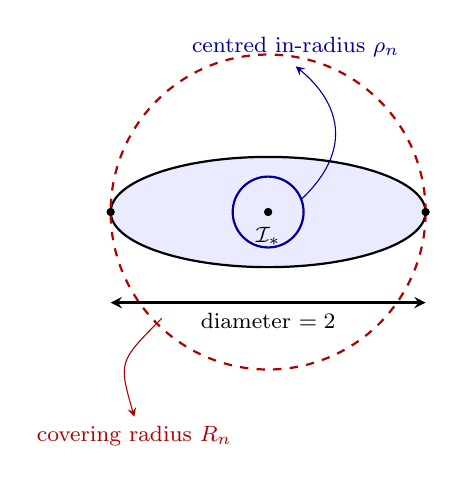
\begin{tikzpicture}[>=stealth]
  \fill[blue!8] (0,0) ellipse (2 and 0.7);
  \draw[thick] (0,0) ellipse (2 and 0.7);
  \draw[thick, blue!60!black] (0,0) circle (0.45);
  \draw[thick, red!70!black, dashed] (0,0) circle (2);
  \fill (0,0) circle (1.5pt) node[below=2pt, font=\footnotesize] {$\mathcal I_*$};
  \draw[->, blue!60!black] (0.42,0.16) .. controls (1.1,0.8) and (0.9,1.4) .. (0.35,1.85) node[anchor=south, font=\footnotesize, blue!60!black] {centred in-radius $\rho_n$};
  \draw[->, red!70!black] (-1.35,-1.35) .. controls (-1.9,-1.9) .. (-1.7,-2.6) node[anchor=north, font=\footnotesize, red!70!black] {covering radius $R_n$};
  \fill (-2,0) circle (1.5pt);
  \fill (2,0) circle (1.5pt);
  \draw[<->, thick] (-2,-1.15) -- (2,-1.15) node[midway, below, font=\footnotesize] {diameter $=2$};
\end{tikzpicture}
\hfil
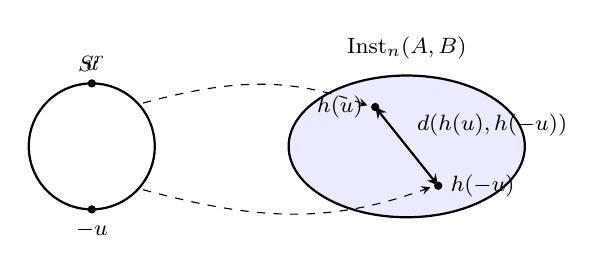
\begin{tikzpicture}[>=stealth]
  \draw[thick] (-2,0) circle (0.8);
  \node[font=\footnotesize] at (-2,1.05) {$S^r$};
  \fill (-2,0.8) circle (1.5pt) node[above=1pt, font=\footnotesize] {$u$};
  \fill (-2,-0.8) circle (1.5pt) node[below=1pt, font=\footnotesize] {$-u$};
  \fill[blue!8] (2,0) ellipse (1.5 and 0.9);
  \draw[thick] (2,0) ellipse (1.5 and 0.9);
  \node[font=\footnotesize] at (2,1.25) {$\Inst_n(A,B)$};
  \fill (1.6,0.5) circle (1.5pt) node[left=1pt, font=\footnotesize] {$h(u)$};
  \fill (2.4,-0.5) circle (1.5pt) node[right=1pt, font=\footnotesize] {$h(-u)$};
  \draw[<->, thick] (1.6,0.5) -- (2.4,-0.5) node[midway, above right, font=\footnotesize] {$d(h(u),h(-u))$};
  \draw[->, dashed] (-1.35,0.55) to[out=15, in=160] (1.5,0.52);
  \draw[->, dashed] (-1.35,-0.55) to[out=-15, in=200] (2.3,-0.52);
\end{tikzpicture}
\caption{The four radius notions of Remark~\ref{rem:radius-terminology}. Left: the centred in-radius $\rho_n$ (largest ball about $\mathcal I_*$ contained in the body), the covering radius $R_n$ (smallest ball about $\mathcal I_*$ containing the body), and the diameter, attained by two points of the body at distance $2$. Right: the antipodal profile: for a continuous map $h:S^r\to\Inst_n(A,B)$, $\alpha_r$ is, up to the factor $1/2$, the largest value of $\min_u d(h(u),h(-u))$ that can be forced; it is governed by antipodal separation, not by balls. The drawing is schematic; the numerical identity $\rho_n+R_n=2$ of Corollary~\ref{cor:complementarity} holds for the exact values of the instrument body, not for a generic convex set.}
\label{fig:radius-notions}
\end{figure}

\begin{proposition}[Monotonicity of profiles, widths, and envelopes]
\label{prop:monotonicity}
For every nonempty metric space $K$,
\[
\alpha_{r+1}(K)\le\alpha_r(K)\qquad(r\ge0),
\]
and if $K$ is compact then $0\le\alpha_r(K)\le\tfrac12\diam(K)$; consequently, if $\alpha_D(K)=0$ then $\alpha_r(K)=0$ for all $r\ge D$. For the instrument body,
\[
\delta_{r+1,\mathrm{inst}}^{\diamond}(A,B)\le\delta_{r,\mathrm{inst}}^{\diamond}(A,B),
\]
and the certified envelopes (Definitions~\ref{def:beta-best} and \ref{def:upper} below) satisfy
\[
\beta_{r+1}^{\mathrm{best},(n)}(A,B)\le\beta_r^{\mathrm{best},(n)}(A,B),\qquad
U_{r+1}^{(n)}(A,B)\le U_r^{(n)}(A,B).
\]
\end{proposition}

\begin{proof}
For the antipodal profile, let $h:S^{r+1}\to K$ be continuous and restrict it to an equatorial copy $S^r\simeq\{(x_0,\dots,x_{r+1})\in S^{r+1}:x_{r+1}=0\}$. The antipodal map on the equator is the ordinary antipodal map on $S^r$, hence
\[
\min_{u\in S^r}d(h(u),h(-u))
\ge\min_{u\in S^{r+1}}d(h(u),h(-u)).
\]
Taking one half and the supremum over all continuous $h:S^{r+1}\to K$ gives $\alpha_r(K)\ge\alpha_{r+1}(K)$. Distances are nonnegative, and $d(h(u),h(-u))\le\diam(K)$ for every $h$ and $u$, so $0\le\alpha_r(K)\le\tfrac12\diam(K)$. If $\alpha_D(K)=0$, the inequality $\alpha_r(K)\le\alpha_D(K)=0$ for $r\ge D$ follows by induction from $\alpha_{r+1}\le\alpha_r$, and $\alpha_r(K)\ge0$ always, so $\alpha_r(K)=0$ for all $r\ge D$.

For the widths, fix any continuous encoder $f:\Inst_n(A,B)\to\mathbb R^r$ and any decoder $g:\mathbb R^r\to\Inst_n(A,B)$, and define $f':\Inst_n(A,B)\to\mathbb R^{r+1}$ by $f'(x)=(f(x),0)$ and $g':\mathbb R^{r+1}\to\Inst_n(A,B)$ by $g'(z_1,\dots,z_{r+1})=g(z_1,\dots,z_r)$. Then $g'\circ f'=g\circ f$ pointwise, so the pair $(f',g')$ achieves the same error at latent dimension $r+1$ that $(f,g)$ achieves at dimension $r$; taking the infimum over $(f,g)$ gives $\delta_{r+1,\mathrm{inst}}^{\diamond}(A,B)\le\delta_{r,\mathrm{inst}}^{\diamond}(A,B)$.

For the lower envelope, the piecewise definition gives $\beta_r^{\mathrm{best},(n)}=1$ on $0\le r\le L_{A,B}^{(n)}$, $\gamma_{A,B}^{(n)}$ on $L_{A,B}^{(n)}<r<D_{A,B}^{(n)}$, and $0$ for $r\ge D_{A,B}^{(n)}$; since $0<\gamma_{A,B}^{(n)}\le1$ (Definition~\ref{def:beta-best}), the sequence is non-increasing.

For the upper envelope, each of the four families of admissible terms in Definition~\ref{def:upper} is monotone in $r$: the constant-code term is independent of $r$; the convex-projection term $2(D_{A,B}^{(n)}-r)/(D_{A,B}^{(n)}-r+1)$ is decreasing in $r$; and the pinching families are defined by threshold conditions $r\ge r_{\mathrm{out}}^{(n)}$ and $r\ge r_{\mathrm{in}}^{(n)}$, so every pinching term admissible at $r$ remains admissible at $r+1$, while further terms may become admissible. Hence every term entering $U_r^{(n)}$ is bounded below by a term entering $U_{r+1}^{(n)}$ (namely the same term, or a smaller newly available one), and $U_{r+1}^{(n)}(A,B)\le U_r^{(n)}(A,B)$.
\end{proof}

Let
\[
\Sstate_{\mathrm{flag}}(B\otimes C_n)
=\Big\{\tau=\sum_{k=1}^n\tau_k\otimes|k\rangle\langle k|:
\tau_k\ge0,\ \sum_{k=1}^n\Tr\tau_k=1\Big\}.
\]
For $\tau\in\Sstate_{\mathrm{flag}}(B\otimes C_n)$ define the replacement instrument $\vec{\mathcal R}_\tau$ by $(\vec{\mathcal R}_\tau)_k(X)=\Tr(X)\tau_k$; each component is completely positive and trace-nonincreasing and the sum is a channel. Write
\[
\RepInst_n(A,B)=\{\vec{\mathcal R}_\tau:\tau\in\Sstate_{\mathrm{flag}}(B\otimes C_n)\}.
\]

\begin{lemma}[Replacement-instrument isometry]
\label{lem:replacement-isometry}
For all flagged states $\tau,\sigma$,
\[
\|\vec{\mathcal R}_\tau-\vec{\mathcal R}_\sigma\|_{\diamond,\mathrm{inst}}
=\|\tau-\sigma\|_1=\sum_{k=1}^n\|\tau_k-\sigma_k\|_1.
\]
\end{lemma}

\begin{proof}
The flagged channel of $\vec{\mathcal R}_\tau$ is the replacement channel $X\mapsto\Tr(X)\tau$. For every reference-assisted input state $\xi$,
\[
(\id\otimes(\widehat{\vec{\mathcal R}_\tau}-\widehat{\vec{\mathcal R}_\sigma}))(\xi)
=\Tr_A(\xi)\otimes(\tau-\sigma),
\]
and $\Tr_A(\xi)$ is a state, so the trace norm equals $\|\tau-\sigma\|_1$ by multiplicativity; the supremum over inputs is unnecessary. The second equality follows from block diagonality in the flag.
\end{proof}

\begin{theorem}[Perfectly separated replacement instruments]
\label{thm:replacement-profile}
Assume $nd_B>1$. Replacement instruments contain a continuous image of $S^{nd_B^2-2}$ whose antipodes have instrument-diamond distance two, and consequently
\[
\alpha_r(\Inst_n(A,B))=1\qquad(0\le r\le nd_B^2-2).
\]
For the replacement family itself the profile is exact:
\[
\alpha_r(\RepInst_n(A,B))=
\begin{cases}
1,&0\le r\le nd_B^2-2,\\
0,&r\ge nd_B^2-1.
\end{cases}
\]
\end{theorem}

\begin{proof}
The real vector space of flag-block-diagonal Hermitian operators on $B\otimes C_n$ has dimension $nd_B^2$; its trace-zero subspace
\[
\mathfrak H_{\mathrm{flag},0}
=\Big\{X=\sum_{k=1}^nX_k\otimes|k\rangle\langle k|:
X_k\in\Herm(B),\ \sum_k\Tr X_k=0\Big\}
\]
has dimension $m:=nd_B^2-1$. Choose any Euclidean norm and let $S(\mathfrak H_{\mathrm{flag},0})\cong S^{m-1}=S^{nd_B^2-2}$ be its unit sphere. For $X$ on the sphere write the Jordan decomposition $X=X_+-X_-$; functional calculus preserves block diagonality and makes $X\mapsto X_+$ continuous. Since $X$ is nonzero and traceless, $t_X:=\Tr X_+=\Tr X_->0$. The map $h(X)=X_+/t_X$ is a continuous map into $\Sstate_{\mathrm{flag}}(B\otimes C_n)$ --- a continuous image of the sphere, and injectivity, which this map may lack, is not required by the antipodal-width arguments --- and $h(-X)=X_-/t_X$ has orthogonal support, so $\|h(X)-h(-X)\|_1=2$. Composing with the replacement embedding of Lemma~\ref{lem:replacement-isometry} gives the claimed sphere of instruments; equatorial restriction supplies every smaller index, and the reverse inequality follows from the diameter bound (Proposition~\ref{prop:diameter}).

For the replacement family above this range, Lemma~\ref{lem:replacement-isometry} identifies $\RepInst_n(A,B)$ affinely and isometrically with the compact convex body of flagged states inside a real affine space of dimension $m=nd_B^2-1$; choose an affine isomorphism of its affine hull with $\mathbb R^{m}$ and compose any continuous $h:S^r\to\RepInst_n(A,B)$ with it. For $r=m$, Borsuk--Ulam~\cite{Matousek2003} applied to $S^{m}\to\mathbb R^{m}$ produces an antipodal collision; for $r>m$, restrict the map to an equatorial $S^m\subset S^r$ first. Every such map therefore has minimum antipodal distance zero, proving the second part of the formula.
\end{proof}

\begin{remark}[In-radius versus antipodal profile]
\label{rem:inradius-vs-alpha}
$\rho_n=2/(nd_Bs)$ certifies a centrally symmetric norm ball in the full direction space $\mathfrak V_{A,B}^{(n)}$, while the sphere $S^{nd_B^2-2}$ via $X\mapsto X_+/\Tr X_+$ certifies a non-linear, antipodally $2$-separated sphere in the replacement body. There is no contradiction between $\rho_n<1$ and $\alpha_r=1$ for $r\le nd_B^2-2$: these are different geometric mechanisms (a ball radius versus an antipodal profile) acting on different subsets of the body. The ball bound governs the intermediate regime, while the replacement sphere governs the small-index regime.
\end{remark}

\begin{theorem}[Full-direction antipodal sphere]
\label{thm:full-direction}
Assume $nd_B>1$, and let $D=D_{A,B}^{(n)}$. For every $0\le r\le D-1$ there exists a continuous map $h:S^r\to\Inst_n(A,B)$ such that
\[
\|h(u)-h(-u)\|_{\diamond,\mathrm{inst}}\ge\frac2{d_A}
\qquad\forall u\in S^r.
\]
Consequently $\alpha_r(\Inst_n(A,B))\ge1/d_A$ for all $0\le r<D$. When $d_A=1$ the separation is $2$, hence $\alpha_r=1$ for all $r<D_{1,B}^{(n)}$, consistent with the exact replacement profile. For $n=1$ the construction restricts to the full-direction sphere of the companion paper~\cite{CompanionChannels}.
\end{theorem}

\begin{proof}
Identify instruments with their normalised flagged Choi operators
\[
J\in\Herm(A_0\otimes B\otimes C_n),\qquad J\ge0,\qquad
\Tr_{B\otimes C_n}J=\frac{I_{A_0}}{d_A},
\]
flag-block-diagonal in $C_n$. The direction space
\[
\mathcal V=\big\{Z\in\Herm(A_0\otimes B\otimes C_n)_{\mathrm{flag}}:\Tr_{B\otimes C_n}Z=0\big\}
\]
has real dimension $D$. Equip $\mathcal V$ with a Euclidean norm and let $S(\mathcal V)\cong S^{D-1}$ be its unit sphere; it suffices to construct the map on $S^{D-1}$, since equatorial restriction supplies every smaller $r$. Fix the uniform flagged state
\[
\tau_0=\frac{I_B}{d_B}\otimes\frac{I_{C_n}}n.
\]
For $Z\in S(\mathcal V)$ write the Jordan decomposition $Z=Z_+-Z_-$ with $Z_+,Z_-\ge0$, $Z_+Z_-=0$; functional calculus preserves flag-block-diagonality. Since $\Tr_{B\otimes C_n}Z=0$,
\[
\Tr_{B\otimes C_n}Z_+=\Tr_{B\otimes C_n}Z_-.
\]
Let $t=\Tr Z_+=\Tr Z_-$. We claim $t>0$: if $t=0$ then $Z_+=0$, so $Z=-Z_-\le0$; but then $\Tr Z=\Tr_{A_0}\Tr_{B\otimes C_n}Z=0$ with $Z\le0$ forces $Z=0$, contradicting $Z\in S(\mathcal V)$. Define the normalised states
\[
\Theta_+=\frac{Z_+}{t},\qquad \Theta_-=\frac{Z_-}{t},
\]
which have orthogonal supports and share the same $A_0$-marginal
\[
\mu:=\Tr_{B\otimes C_n}\Theta_+=\Tr_{B\otimes C_n}\Theta_-.
\]
If $d_A=1$ the marginal condition is automatic ($A_0$ is one-dimensional and $\mu=1$), and we set $J^+(Z)=\Theta_+$, $J^-(Z)=\Theta_-$. Otherwise put $\lambda=1/d_A$. Since $\mu$ is a state on $A_0$, $\mu\le I_{A_0}$, hence $\lambda\mu\le I_{A_0}/d_A$. Define the correction state
\[
\nu=\frac{\frac{I_{A_0}}{d_A}-\lambda\mu}{1-\lambda}
=\frac{I_{A_0}-\mu}{d_A-1}\ge0,
\qquad \Tr\nu=1,
\]
and set
\[
J^+(Z)=\lambda\Theta_++(1-\lambda)\nu\otimes\tau_0,\qquad
J^-(Z)=\lambda\Theta_-+(1-\lambda)\nu\otimes\tau_0.
\]
Both $J^\pm(Z)$ are positive and flag-block-diagonal --- the $\Theta_\pm$ summands inherit flag-block-diagonality from $Z$ through the Jordan decomposition, and the correction term $\nu\otimes\tau_0$ is flag-block-diagonal because $\tau_0$ is diagonal in the fixed flag basis --- with $A_0$-marginal
\[
\lambda\mu+(1-\lambda)\nu=\frac{I_{A_0}}{d_A},
\]
so each is the normalised flagged Choi operator of an instrument; let $h(Z)$ be the instrument with Choi operator $J^+(Z)$. For $-Z$ the positive and negative parts are interchanged while $t$ and $\mu$ are unchanged, so $\nu$ is unchanged and $h(-Z)$ is the instrument with Choi operator $J^-(Z)$. The Choi difference is
\[
J^+(Z)-J^-(Z)=\lambda(\Theta_+-\Theta_-)
\]
(with $\lambda=1$ when $d_A=1$), and since $\Theta_+,\Theta_-$ are states with orthogonal supports,
\[
\|J^+(Z)-J^-(Z)\|_1=2\lambda=\frac2{d_A}.
\]
For any Hermiticity-preserving tuple $\vD$,
\[
\|\vD\|_{\diamond,\mathrm{inst}}\ge\|\Jhat_{\widehat{\vD}}\|_1,
\]
because testing the flagged map on the maximally entangled input state produces its normalised Choi operator. Therefore
\[
\|h(Z)-h(-Z)\|_{\diamond,\mathrm{inst}}\ge\frac2{d_A}.
\]
Finally, $Z\mapsto Z_+$ is continuous on Hermitian operators and $t=\Tr Z_+$ is continuous and strictly positive on the compact unit sphere $S(\mathcal V)$, hence bounded away from zero there; so $Z\mapsto J^+(Z)$ is continuous. Equatorial restriction proves the theorem for all $0\le r\le D-1$.
\end{proof}

\begin{remark}[Tunable mixing parameter]
\label{rem:tunable-lambda}
In the proof of Theorem~\ref{thm:full-direction}, the mixing parameter may be chosen as a function of $Z$: since $\mu=\mu(Z)$ is a state on $A_0$ we have $\|\mu\|_\infty\in[1/d_A,1]$, and $I_{A_0}/d_A-\lambda\mu\ge0$ holds if and only if $\lambda\le1/(d_A\|\mu\|_\infty)$. Taking $\lambda(Z)=1/(d_A\|\mu(Z)\|_\infty)\in[1/d_A,1]$ therefore increases the pointwise separation to
\[
\|J^+(Z)-J^-(Z)\|_1=\frac{2}{d_A\|\mu(Z)\|_\infty}\ge\frac2{d_A},
\]
with $\lambda=1$ exactly when $\mu(Z)=I_{A_0}/d_A$, in which case no correction state is needed. The uniform certificate $\alpha_r\ge1/d_A$ is unchanged. The proof of Theorem~\ref{thm:full-direction} uses the constant value $\lambda=1/d_A$, which makes continuity of the construction immediate; near points with $\mu(Z)=I_{A_0}/d_A$, a variable quotient $\nu(Z)$ would require a separate gluing argument.
\end{remark}

\begin{corollary}[Antipodal cutoff at affine dimension]
\label{cor:cutoff}
Assume $nd_B>1$. Then $\alpha_r(\Inst_n(A,B))=0$ for all $r\ge D_{A,B}^{(n)}$.
\end{corollary}

\begin{proof}
Choose affine coordinates $c:\mathfrak A_{A,B}^{(n)}\to\mathbb R^{D}$ (an affine isomorphism, hence injective). For any continuous $h:S^r\to\Inst_n(A,B)$ with $r\ge D$, restrict to an equatorial $S^D\subset S^r$; Borsuk--Ulam applied to $c\circ h:S^D\to\mathbb R^D$ gives $u$ with $c(h(u))=c(h(-u))$, hence $h(u)=h(-u)$ by injectivity. Thus $\alpha_D=0$, and monotonicity (Proposition~\ref{prop:monotonicity}) extends this to all $r\ge D$.
\end{proof}

\begin{theorem}[Observable antipodal sphere]
\label{thm:observable}
Assume either (i) $n\ge2$ and $d_A\ge2$, or (ii) $n=1$, $d_A\ge2$, $d_B\ge2$. Then there exists a continuous map $h:S^{d_A^2-2}\to\Inst_n(A,B)$ whose antipodal images have instrument-diamond distance $2$; consequently
\[
\alpha_r(\Inst_n(A,B))=1\qquad(0\le r\le d_A^2-2).
\]
For $n=1$ this is the observable sphere of the channel-level companion paper~\cite{CompanionChannels}. The construction is a continuous image of the sphere and may fail to be injective: $H$ and its positive scalar multiples define the same instrument. Injectivity is not required by the width arguments.
\end{theorem}

\begin{proof}
First suppose $n\ge2$. Fix a unit vector $|b_0\rangle\in B$ and let $\sigma=|b_0\rangle\langle b_0|$. For $H\in\Herm_0(A)$, $H\neq0$, define
\[
K(H)=\frac{H}{\|H\|_\infty},\qquad E_\pm(H)=\frac{I_A\pm K(H)}2.
\]
Then $E_\pm(H)\ge0$ and $E_+(H)+E_-(H)=I_A$. Define an instrument by
\[
\mathcal I^H_1(X)=\Tr(E_+(H)X)\sigma,\qquad
\mathcal I^H_2(X)=\Tr(E_-(H)X)\sigma,\qquad
\mathcal I^H_k(X)=0\ (k\ge3);
\]
the sum is the replacement channel $X\mapsto\Tr(X)\sigma$, so $\mathcal I^H\in\Inst_n(A,B)$. Since $\|K(H)\|_\infty=1$, $K(H)$ has a unit eigenvector $|\psi\rangle$ with eigenvalue $\varepsilon\in\{+1,-1\}$. Then
\[
\Tr(E_{\varepsilon}(H)|\psi\rangle\langle\psi|)=1,\qquad
\Tr(E_{-\varepsilon}(H)|\psi\rangle\langle\psi|)=0,
\]
where $E_{+1}(H)=E_+(H)$ and $E_{-1}(H)=E_-(H)$; since $E_\pm(-H)=E_\mp(H)$, the two effects are exchanged for $-H$. Hence the flagged outputs of $\mathcal I^H$ and $\mathcal I^{-H}$ on the input $|\psi\rangle\langle\psi|$ are $\sigma\otimes|1\rangle\langle1|$ and $\sigma\otimes|2\rangle\langle2|$ in one order or the other, which are orthogonal, so their trace norm difference is $2$; by the diameter bound the instrument distance is exactly $2$. The map $H\mapsto H/\|H\|_\infty$ is continuous on the Euclidean unit sphere of $\Herm_0(A)\cong\mathbb R^{d_A^2-1}$, so the construction gives a continuous image of $S^{d_A^2-2}$ with antipodal distance $2$; equatorial restriction gives the result for all $0\le r\le d_A^2-2$.

For $n=1$ and $d_B\ge2$, choose two orthogonal output states $\sigma_+,\sigma_-$ and define the channel
\[
\Phi^H(X)=\Tr(E_+(H)X)\sigma_++\Tr(E_-(H)X)\sigma_-.
\]
The same eigenvector witness gives orthogonal outputs $\sigma_+$ and $\sigma_-$, hence distance $2$, and the continuity argument is identical.
\end{proof}

\begin{proposition}[Orthogonal join of flagged state spheres]
\label{prop:join}
Let $W_1,\dots,W_\ell$ be pairwise orthogonal flag-block-diagonal subspaces of $B\otimes C_n$, and suppose that continuous maps $h_i:S^{r_i}\to\Sstate_{\mathrm{flag}}(B\otimes C_n)$ take values in states supported on $W_i$ and satisfy
\[
\|h_i(u)-h_i(-u)\|_1=2\qquad(u\in S^{r_i}).
\]
Then there is a continuous map $H:S^{\sum_i r_i+\ell-1}\to\Sstate_{\mathrm{flag}}(B\otimes C_n)$ with
\[
\|H(y)-H(-y)\|_1=2
\]
for every $y$. Composing with the replacement-instrument embedding gives the same antipodal separation in instrument diamond norm.
\end{proposition}

\begin{proof}
View the domain sphere as the unit sphere of $\bigoplus_{i=1}^{\ell}\mathbb R^{r_i+1}$. For a point $y=(y_1,\dots,y_\ell)$ on it, write
$\lambda_i=\|y_i\|_2^2$ and, on the blocks with $y_i\neq0$, $u_i=y_i/\|y_i\|_2$; then define
\[
H(y)=\sum_{i:y_i\neq0}\lambda_i\,h_i(u_i),
\]
reading the $i$-th summand as zero when $y_i=0$. The weights satisfy $\sum_i\lambda_i=1$, so $H(y)$ is a flagged state. Continuity at points where some $y_i=0$ follows because the trace norm of the $i$-th summand is $\|\lambda_i h_i(u_i)\|_1=\lambda_i\to0$ as $y_i\to0$, uniformly in the direction $u_i$. Because the supports $W_i$ are pairwise orthogonal, the difference $H(y)-H(-y)$ is block diagonal with respect to $\bigoplus_iW_i$, so
\[
\|H(y)-H(-y)\|_1
=\sum_i\lambda_i\|h_i(u_i)-h_i(-u_i)\|_1
=2\sum_i\lambda_i=2.
\]
Lemma~\ref{lem:replacement-isometry} transfers the equality to replacement instruments.
\end{proof}

\begin{proposition}[Instrument-level join with replacement spheres]
\label{prop:join-inst}
Let $W\subseteq B\otimes C_n$ be a flag-block-diagonal subspace. Let $h:S^{r_1}\to\Inst_n(A,B)$ be continuous and such that
\begin{enumerate}[leftmargin=*,itemsep=2pt]
\item for every input state $\rho$ on $A_0\otimes A$ and every $u\in S^{r_1}$, the flagged output $(\id_{A_0}\otimes\widehat{h(u)})(\rho)$ is supported on $A_0\otimes W$, and
\item $\|h(u)-h(-u)\|_{\diamond,\mathrm{inst}}=2$ for every $u\in S^{r_1}$.
\end{enumerate}
Let $\tau:S^{r_2}\to\Sstate_{\mathrm{flag}}(B\otimes C_n)$ be continuous, take values in states supported on the per-block orthogonal complement $W^{\perp}$, and satisfy $\|\tau(v)-\tau(-v)\|_1=2$ for every $v\in S^{r_2}$. Then, on the unit sphere of $\mathbb R^{r_1+1}\oplus\mathbb R^{r_2+1}$,
\[
\mathcal I(y)=\|y_1\|_2^2\,h\!\left(\frac{y_1}{\|y_1\|_2}\right)
+\|y_2\|_2^2\,\vec{\mathcal R}_{\tau(y_2/\|y_2\|_2)}
\]
(with a summand read as zero when the corresponding coordinate block vanishes) defines a continuous map $S^{r_1+r_2+1}\to\Inst_n(A,B)$ with
\[
\|\mathcal I(y)-\mathcal I(-y)\|_{\diamond,\mathrm{inst}}=2\qquad(y\in S^{r_1+r_2+1}).
\]
\end{proposition}

\begin{proof}
Both summands are convex combinations of instruments, hence instruments, so $\mathcal I(y)\in\Inst_n(A,B)$; the instrument body is bounded (every flagged channel has diamond norm $1$), so each summand tends to zero in norm as its weight tends to zero, uniformly over the sphere, which gives continuity on the coordinate spheres $\{y_i=0\}$ exactly as in Proposition~\ref{prop:join}. Fix $y$ and write $\lambda=\|y_1\|_2^2$, $u=y_1/\|y_1\|_2$, $v=y_2/\|y_2\|_2$ where the corresponding blocks are nonzero. If $\lambda=0$ the claim reduces to the replacement pair, at distance $2$ by Lemma~\ref{lem:replacement-isometry}. Otherwise set $\vD_1=h(u)-h(-u)$ and $\vD_2=\vec{\mathcal R}_{\tau(v)}-\vec{\mathcal R}_{\tau(-v)}$, so that $\mathcal I(y)-\mathcal I(-y)=\lambda\vD_1+(1-\lambda)\vD_2$. The set of input states is compact and $\rho\mapsto\|(\id\otimes\vD_1)(\rho)\|_1$ is continuous with supremum $\|\vD_1\|_{\diamond,\mathrm{inst}}=2$, so there is an input state $\rho_*$ with $\|(\id\otimes\vD_1)(\rho_*)\|_1=2$. For this same input, Lemma~\ref{lem:replacement-isometry} gives $(\id\otimes\vD_2)(\rho_*)=\Tr_A(\rho_*)\otimes(\tau(v)-\tau(-v))$, of trace norm $\|\tau(v)-\tau(-v)\|_1=2$, independently of $\rho_*$. By (i) applied to $h(u)$ and $h(-u)$, the Hermitian operator $(\id\otimes\vD_1)(\rho_*)$ is supported on $A_0\otimes W$, while $(\id\otimes\vD_2)(\rho_*)$ is supported on $A_0\otimes W^{\perp}$; orthogonal supports make the trace norm additive, so
\[
\big\|(\id\otimes(\mathcal I(y)-\mathcal I(-y)))(\rho_*)\big\|_1
=\lambda\cdot2+(1-\lambda)\cdot2=2.
\]
Hence $\|\mathcal I(y)-\mathcal I(-y)\|_{\diamond,\mathrm{inst}}\ge2$, and the reverse inequality is the diameter bound (Proposition~\ref{prop:diameter}).
\end{proof}

\begin{remark}[Why the join carries at most one input-dependent sphere]
\label{rem:join-one-observable}
Proposition~\ref{prop:join-inst} joins one \emph{input-dependent} sphere with replacement spheres: the replacement components attain their maximal separation $2$ on \emph{every} input, so an input that exposes the input-dependent component simultaneously exposes all of them. Two input-dependent components could not be joined by this mechanism, since their separating inputs (eigenvectors of the respective observables) vary with the sphere parameter and need not coincide; this is why exactly one observable sphere enters Corollary~\ref{cor:join-dimension} below.
\end{remark}

\begin{corollary}[Observable--replacement join dimension]
\label{cor:join-dimension}
Under the hypotheses of Theorem~\ref{thm:observable}, the flagged outputs of the observable sphere are supported on the flagged subspace
\[
W_{\mathrm{obs}}=\operatorname{span}\{|b_0\rangle\otimes|1\rangle,\ |b_0\rangle\otimes|2\rangle\}
\]
in the case $n\ge2$ (with the pure state $\sigma=|b_0\rangle\langle b_0|$), and on the two-dimensional flagged subspace $W_{\mathrm{obs}}=\operatorname{span}\{|\varphi_+\rangle,|\varphi_-\rangle\}$ in the case $n=1$, where $\sigma_\pm=|\varphi_\pm\rangle\langle\varphi_\pm|$ are the two orthogonal output states of the channel construction. Let $W_{\mathrm{obs}}^{\perp}$ denote the per-block orthogonal complement of $W_{\mathrm{obs}}$: when $n\ge2$ its first two blocks are $\{|b_0\rangle\}^{\perp}\subseteq B$ and its remaining $n-2$ blocks are all of $B$; when $n=1$ it is the orthogonal complement of $W_{\mathrm{obs}}$ in $B$. The real vector space of flag-block-diagonal Hermitian operators supported on $W_{\mathrm{obs}}^{\perp}$ has dimension
\[
N_{\mathrm{join}}=
\begin{cases}
2(d_B-1)^2+(n-2)d_B^2,&n\ge2,\\
(d_B-2)^2,&n=1.
\end{cases}
\]
If $N_{\mathrm{join}}\ge2$, then
\[
\alpha_r(\Inst_n(A,B))=1\qquad(0\le r\le d_A^2+N_{\mathrm{join}}-3).
\]
For $n=1$ this is the observable--replacement join of the companion paper~\cite{CompanionChannels}.
\end{corollary}

\begin{proof}
The observable sphere $h:S^{d_A^2-2}\to\Inst_n(A,B)$ of Theorem~\ref{thm:observable} is continuous and has antipodal instrument-diamond distance $2$; on every input $\rho$, each outcome component of its flagged output is a positive operator on $A_0$ tensored with $\sigma\otimes|k\rangle\langle k|$, $k\in\{1,2\}$ (respectively with $\sigma_+$ or $\sigma_-$ when $n=1$), and the remaining outcomes vanish, so all flagged outputs are supported on $A_0\otimes W_{\mathrm{obs}}$, i.e.\ hypothesis (i) of Proposition~\ref{prop:join-inst} holds with $W=W_{\mathrm{obs}}$. The per-block complement $W_{\mathrm{obs}}^{\perp}$ is itself flag-block-diagonal, and the Jordan construction of Theorem~\ref{thm:replacement-profile}, applied to the traceless part of the real vector space of flag-block-diagonal Hermitian operators supported on $W_{\mathrm{obs}}^{\perp}$, produces a continuous sphere $\tau:S^{N_{\mathrm{join}}-2}\to\Sstate_{\mathrm{flag}}(B\otimes C_n)$ of states supported on $W_{\mathrm{obs}}^{\perp}$ with $\|\tau(v)-\tau(-v)\|_1=2$; the condition $N_{\mathrm{join}}\ge2$ is exactly nonemptiness of this sphere. Proposition~\ref{prop:join-inst} joins the two spheres into a continuous map
\[
S^{(d_A^2-2)+(N_{\mathrm{join}}-2)+1}=S^{d_A^2+N_{\mathrm{join}}-3}\longrightarrow\Inst_n(A,B)
\]
with antipodal instrument-diamond distance $2$; equatorial restriction supplies every smaller index, and $\alpha_r\le1$ always by the diameter bound (Proposition~\ref{prop:diameter}).
\end{proof}

\begin{remark}[Structured partitions]
\label{rem:partitions}
The $\ell$-fold join of Proposition~\ref{prop:join} may also be applied to arbitrary pairwise orthogonal output--flag blocks $(B_i,n_i)$ with $\sum_ib_i\le d_B$, $\sum_in_i=n$, producing a sphere of dimension $\sum_i(n_ib_i^2-1)-1$ whenever $n_ib_i^2\ge2$ for every retained block. Taking one block with $b_1=d_B$, $n_1=n$ recovers the leading dimension $nd_B^2-2$; no partition improves Theorem~\ref{thm:replacement-profile}.
\end{remark}

\begin{definition}[Certified one-sphere dimension]
\label{def:one-sphere}
Let
\[
L_{\mathrm{rep}}=nd_B^2-2,
\]
valid whenever $nd_B>1$. If either $n\ge2,d_A\ge2$, or $n=1,d_A\ge2,d_B\ge2$, set $L_{\mathrm{obs}}=d_A^2-2$; otherwise set $L_{\mathrm{obs}}=-1$. If the observable sphere is valid and $N_{\mathrm{join}}\ge2$ (Corollary~\ref{cor:join-dimension}), set $L_{\mathrm{join}}=d_A^2+N_{\mathrm{join}}-3$; otherwise $L_{\mathrm{join}}=-1$. Finally define
\[
L_{A,B}^{(n)}
=\min\Big\{D_{A,B}^{(n)}-1,\ \max\{L_{\mathrm{rep}},L_{\mathrm{obs}},L_{\mathrm{join}}\}\Big\},
\]
where invalid terms ($-1$) are ignored. If $d_A=1$, the observable and join terms are invalid and $L_{1,B}^{(n)}=nd_B^2-2=D_{1,B}^{(n)}-1$.
\end{definition}

\begin{definition}[Certified lower envelope]
\label{def:beta-best}
Assume $nd_B>1$. Let
\[
\rho_n=\frac{2}{nd_B\min\{d_A,d_B\}},\qquad
\gamma_{A,B}^{(n)}=\max\Big\{\rho_n,\frac1{d_A}\Big\}.
\]
Define
\[
\beta_r^{\mathrm{best},(n)}(A,B)=
\begin{cases}
1,&0\le r\le L_{A,B}^{(n)},\\[3pt]
\gamma_{A,B}^{(n)},&L_{A,B}^{(n)}<r<D_{A,B}^{(n)},\\[6pt]
0,&r\ge D_{A,B}^{(n)}.
\end{cases}
\]
When $L_{A,B}^{(n)}=D_{A,B}^{(n)}-1$ the middle range is empty (this is always the case for $d_A=1$). Since $nd_Bs\ge2$ and $d_A\ge1$, one has $0<\gamma_{A,B}^{(n)}\le1$, so the displayed envelope is non-increasing in $r$. Every component is rigorously certified by Theorems~\ref{thm:replacement-profile}, \ref{thm:full-direction}, \ref{thm:observable}, Corollary~\ref{cor:join-dimension}, and Theorem~\ref{thm:ball}.
\end{definition}

\begin{remark}[Resource interpretation of the two breakpoints]
\label{rem:breakpoints}
The two breakpoints of the envelope have a direct resource interpretation. A flagged output state has $nd_B^2-1$ affine parameters, while an input-dependent instrument has $d_A^2(nd_B^2-1)$. The first regime ($r\le L_{A,B}^{(n)}$) is already obstructed by preparing and recording one classical--quantum output state --- augmented by the observable constructions, which obstruct input-dependent effect readout even when the output state is fixed. The second regime concerns the additional dependence of all outcome branches on the input operator. Increasing the number of outcomes therefore has two opposite effects: it linearly enlarges the global representation space, while dividing the local positivity margin of the uniform instrument by $n$.
\end{remark}

\begin{remark}[Two mechanisms behind the intermediate floor]
\label{rem:gamma-mechanisms}
The intermediate floor $\gamma_{A,B}^{(n)}=\max\{\rho_n,1/d_A\}$ combines two certificates of different geometric origin, and the maximum is the correct combination because each term is individually a valid lower bound on every width in the intermediate regime. The term $\rho_n=2/(nd_Bs)$ is a local statement: a ball of radius $\rho_n$ about the uniform instrument exists, and the antipodal pairs inside a centrally symmetric ball certify error at least $\rho_n$ via the radial map (Corollary~\ref{cor:intrinsic}); it decays with $n$ because the uniform trace budget is split among $n$ outcomes. The term $1/d_A$ is a global statement: a sphere spanning all $D_{A,B}^{(n)}$ directions of the body exists whose antipodes are separated by $2/d_A$ (Theorem~\ref{thm:full-direction}); the value $1/d_A$ is the largest mixing weight at which two orthogonal flagged Choi states with a common input marginal can be completed to instruments uniformly over all directions, the direction-dependent optimum $1/(d_A\|\mu(Z)\|_\infty)$ of Remark~\ref{rem:tunable-lambda} collapsing to $1/d_A$ exactly at the maximally mixed marginal. The two terms trade off at $n\approx2d_A/(d_B\min\{d_A,d_B\})$: below this threshold the ball term dominates the maximum, above it the input-dimension term $1/d_A$ is the floor; in particular, whenever $d_A\le d_B$ the floor is $1/d_A$ for every $n\ge2$. This is the geometric reason the intermediate obstruction carries an $n$-independent component. The $n=1$ value $\gamma_{A,B}^{(1)}=\max\{2/(d_B\min\{d_A,d_B\}),1/d_A\}$ is the intermediate envelope value of the companion paper~\cite{CompanionChannels}.
\end{remark}

\section{Compression widths: upper bounds and exact thresholds}
\label{sec:widths}

The spheres of the preceding section certify that certain widths are large; this section supplies the matching upper bounds and the exact threshold where the width collapses to zero. The two sides bracket every intermediate width in an explicit interval. The widths defined below are continuous-encoding analogues of the classical Kolmogorov $n$-widths of a compact set in a normed space~\cite{Pinkus1985}, with the linear subspaces of the classical theory replaced by arbitrary continuous images of $\mathbb R^r$.

\begin{convention}[Continuous encoding, unrestricted decoding]
\label{conv:decoder}
Throughout the compression-width results, an encoder is required to be continuous while the decoder is unrestricted unless explicitly stated otherwise. This convention is essential for the Helly-type upper bounds; where a continuous decoder is available we state this separately.
\end{convention}

\begin{definition}[Euclidean instrument width]
\label{def:width}
\[
\delta_{r,\mathrm{inst}}^{\diamond}(A,B)
=\inf_{\substack{f:\Inst_n(A,B)\to\mathbb R^r\ \text{continuous}\\ g:\mathbb R^r\to\Inst_n(A,B)}}
\sup_{\mathcal I\in\Inst_n(A,B)}
\|g(f(\mathcal I))-\mathcal I\|_{\diamond,\mathrm{inst}}.
\]
For compact metric $K\subseteq L$ we also use $\delta_r^{\mathrm c}(K;L)$, the analogous width with continuous encoders into $\mathbb R^r$ and arbitrary (not necessarily continuous) decoders into $L$.
\end{definition}

\begin{remark}[Decoder codomain does not weaken the lower bounds]
\label{rem:decoder-codomain}
Since $\RepInst_n(A,B)\subset\Inst_n(A,B)\subset\mathfrak A_{A,B}^{(n)}$, and the triangle inequality $\|h(u)-\Psi\|_{\diamond,\mathrm{inst}}+\|h(-u)-\Psi\|_{\diamond,\mathrm{inst}}\ge\|h(u)-h(-u)\|_{\diamond,\mathrm{inst}}$ holds for every $\Psi$ in the ambient vector space $\bigoplus_k\Lin(A,B)$, the lower bounds of Corollaries~\ref{cor:intrinsic} and \ref{cor:euclidean} (stated below) are proved for decoders with values in the full affine space $\mathfrak A_{A,B}^{(n)}$ --- a strictly stronger statement than for instrument-valued decoders. Hence
\begin{align*}
\beta_r^{\mathrm{best},(n)}(A,B)
&\le\delta_r^{\mathrm c}\big(\Inst_n(A,B);\mathfrak A_{A,B}^{(n)}\big)\\
&\le\delta_r^{\mathrm c}\big(\Inst_n(A,B);\Inst_n(A,B)\big)
=\delta_{r,\mathrm{inst}}^{\diamond}(A,B)
\le U_r^{(n)}(A,B).
\end{align*}
Allowing unphysical affine decoders cannot circumvent the certified lower envelope; and because the optimal constant-code centre $\mathcal I_*$ is itself an instrument (Theorem~\ref{thm:covering}), the constant-code width coincides over both codomains (Corollary~\ref{cor:constant-code}), so every upper bound of this paper is admissible with a physical instrument decoder. The same codomain convention underlies the Hermiticity-preserving trace-preserving decoder bounds of the companion paper~\cite{CompanionChannels}.
\end{remark}

\begin{corollary}[Certified width bracket]
\label{cor:bracket}
Assume $nd_B>1$. For $0\le r<D_{A,B}^{(n)}$,
\[
\beta_r^{\mathrm{best},(n)}(A,B)
\le\delta_{r,\mathrm{inst}}^{\diamond}(A,B)
\le U_r^{(n)}(A,B),
\]
where $U_r^{(n)}$ is defined in Definition~\ref{def:upper}. For $r\ge D_{A,B}^{(n)}$ the width is zero.
\end{corollary}

\begin{proof}
For $0\le r\le L_{A,B}^{(n)}$ the replacement sphere, observable sphere, or observable--replacement join supplies a continuous map $h:S^r\to\Inst_n(A,B)$ with antipodal distance $2$; composing with any continuous encoder $f$ gives $f\circ h:S^r\to\mathbb R^r$, and Borsuk--Ulam produces $u$ with $f(h(u))=f(h(-u))$. The decoder returns one reconstruction for the pair, and the triangle inequality forces error at least $1=\beta_r^{\mathrm{best},(n)}$. The argument applies verbatim to decoders valued in the ambient affine space $\mathfrak A_{A,B}^{(n)}$ (Remark~\ref{rem:decoder-codomain}), which only strengthens the lower bound. For $L_{A,B}^{(n)}<r<D_{A,B}^{(n)}$, two independent certificates hold: the centred ball gives antipodal separation $2\rho_n$ (via the radial map of Corollary~\ref{cor:intrinsic}, which needs only $r+1\le D_n$), and Theorem~\ref{thm:full-direction} gives separation $2/d_A$. Choose the radial map if $\rho_n\ge1/d_A$ and the full-direction map if $1/d_A\ge\rho_n$; the chosen map has separation $2\gamma_{A,B}^{(n)}$, hence error at least $\gamma_{A,B}^{(n)}$. The upper terms are Theorem~\ref{thm:covering}, Theorem~\ref{thm:pinching} and Proposition~\ref{prop:convex} (stated below); exact reconstruction for $r\ge D_{A,B}^{(n)}$ is Theorem~\ref{thm:zero-error}.
\end{proof}

For a Hausdorff latent space $Y$, recall the deleted product
\[
F_2(Y)=\{(y_0,y_1)\in Y^2:y_0\neq y_1\}
\]
with the involution exchanging the two entries, and let
\[
\coind F_2(Y)
=\sup\big\{k\ge0:\exists\ \text{equivariant}\ S^k\to F_2(Y)\big\},
\]
with value $-1$ when $F_2(Y)$ is empty and possible value $+\infty$. For a metric space $Y$, $F_2(Y)$ carries the subspace topology of $Y^2$ and the free $\mathbb Z_2$-action; Hausdorffness is not needed for the deleted product itself, but is natural to make the diagonal closed. If $\coind F_2(Y)=+\infty$, no integer $q$ satisfies $q>\coind F_2(Y)$ and the corollary below is vacuous. For $r\ge1$, if $Y$ admits a continuous injection $\jmath:Y\to\mathbb R^r$, the normalised difference map
\[
(y_0,y_1)\longmapsto\frac{\jmath(y_0)-\jmath(y_1)}{\|\jmath(y_0)-\jmath(y_1)\|_2}
\]
is continuous and equivariant $F_2(Y)\to S^{r-1}$, so by Borsuk--Ulam~\cite{Matousek2003}, $\coind F_2(Y)\le r-1$.

\begin{corollary}[Intrinsic latent-space instrument hierarchy]
\label{cor:intrinsic}
Assume $nd_B>1$. Let $Y$ be Hausdorff and let $q\in\mathbb N_0$ satisfy
\[
q>\coind F_2(Y).
\]
Then every continuous encoder $\operatorname{Enc}:\Inst_n(A,B)\to Y$ and every decoder $\operatorname{Dec}:Y\to\mathfrak A_{A,B}^{(n)}$ satisfy
\[
\sup_{\mathcal I\in\Inst_n(A,B)}
\|\operatorname{Dec}(\operatorname{Enc}(\mathcal I))-\mathcal I\|_{\diamond,\mathrm{inst}}
\ge\beta_q^{\mathrm{best},(n)}(A,B).
\]
\end{corollary}

\begin{proof}
If $q\ge D_{A,B}^{(n)}$, then $\beta_q^{\mathrm{best},(n)}(A,B)=0$ and the claimed inequality is trivial; assume henceforth $q<D_{A,B}^{(n)}$. If $0\le q\le L_{A,B}^{(n)}$, restrict the perfectly separated sphere supplied by Theorem~\ref{thm:replacement-profile}, Theorem~\ref{thm:observable}, or Corollary~\ref{cor:join-dimension} to an equatorial $S^q$. If $L_{A,B}^{(n)}<q<D_{A,B}^{(n)}$, then $q+1\le D_{A,B}^{(n)}$; choose a $(q+1)$-dimensional subspace $W\subseteq\mathfrak V_{A,B}^{(n)}$ and use the radial map
\[
h(u)=\mathcal I_*+\rho_n\frac{u}{\|u\|_{\diamond,\mathrm{inst}}}
\]
on an auxiliary Euclidean sphere $S^q\subset W$ (the denominator $\|u\|_{\diamond,\mathrm{inst}}$ is a continuous and strictly positive function on the compact Euclidean sphere, so the normalisation is continuous). Theorem~\ref{thm:ball} makes the radial map instrument-valued with antipodal separation $2\rho_n$, and Theorem~\ref{thm:full-direction} independently supplies a map with separation $2/d_A$; choose the radial map when $\rho_n\ge1/d_A$ and the full-direction map otherwise, so that the chosen map has antipodal separation $2\gamma_{A,B}^{(n)}$. In both regimes, if the two latent codes $\operatorname{Enc}(h(u))$ and $\operatorname{Enc}(h(-u))$ were distinct for every $u$, then $u\mapsto(\operatorname{Enc}(h(u)),\operatorname{Enc}(h(-u)))$ would be an equivariant map $S^q\to F_2(Y)$, contradicting the coindex hypothesis. An antipodal pair therefore has one code; the decoder returns one reconstruction for it, and the triangle inequality gives half the separation, namely $\beta_q^{\mathrm{best},(n)}(A,B)$.
\end{proof}

\begin{corollary}[Continuous instrument-compression hierarchy]
\label{cor:euclidean}
Assume $nd_B>1$, and let $Y$ admit a continuous injection into $\mathbb R^r$. Then, for every continuous encoder $\operatorname{Enc}:\Inst_n(A,B)\to Y$ and every decoder $\operatorname{Dec}:Y\to\mathfrak A_{A,B}^{(n)}$,
\[
\sup_{\mathcal I\in\Inst_n(A,B)}
\|\operatorname{Dec}(\operatorname{Enc}(\mathcal I))-\mathcal I\|_{\diamond,\mathrm{inst}}
\ge\beta_r^{\mathrm{best},(n)}(A,B).
\]
\end{corollary}

\begin{proof}
If $r=0$ then $Y$ has at most one point and $F_2(Y)=\emptyset$ has coindex $-1$; if $r\ge1$ the normalised difference map gives $\coind F_2(Y)\le r-1$ as above. Apply Corollary~\ref{cor:intrinsic} with $q=r$.
\end{proof}

\begin{theorem}[Zero-error threshold, with continuous decoding at the threshold]
\label{thm:zero-error}
For Euclidean latent spaces and under Convention~\ref{conv:decoder},
\[
\delta_{r,\mathrm{inst}}^{\diamond}(A,B)=0
\quad\Longleftrightarrow\quad
r\ge D_{A,B}^{(n)}.
\]
Moreover, for every $r\ge D_{A,B}^{(n)}$, exact decoding may be chosen continuous.
\end{theorem}

\begin{proof}
For $r\ge D_{A,B}^{(n)}$, choose affine coordinates $c:\mathfrak A_{A,B}^{(n)}\to\mathbb R^{D}$ (an affine isomorphism) and restrict to the compact convex body $K=\Inst_n(A,B)$; its image $C=c(K)\subset\mathbb R^{D}$ is compact and convex. The encoder is $f=c|_K$, padded with zeros if $r>D$. Let $\Pi_C:\mathbb R^{D}\to C$ be the Euclidean nearest-point projection: for a nonempty closed convex subset of Euclidean space the metric projection is single-valued and $1$-Lipschitz, hence continuous. Define the decoder $g(z)=c^{-1}(\Pi_C(z_1,\dots,z_D))$, ignoring any padding. Then $g(f(x))=x$ for every $x\in K$ and $g$ is continuous. For the converse, if $r<D_{A,B}^{(n)}$ then $\beta_r^{\mathrm{best},(n)}(A,B)>0$ (Corollary~\ref{cor:euclidean}), so exact reconstruction is impossible even with an arbitrary decoder; the collision $f(h(u))=f(h(-u))$ forces one decoder value to cover two distinct instruments, using only that the \emph{code values coincide}, with no regularity assumption on the decoder.
\end{proof}

\begin{proposition}[Convex-projection instrument bound]
\label{prop:convex}
For $0\le r\le D_{A,B}^{(n)}$,
\[
\delta_{r,\mathrm{inst}}^{\diamond}(A,B)
\le\frac{2(D_{A,B}^{(n)}-r)}{D_{A,B}^{(n)}-r+1}.
\]
\end{proposition}

\begin{proof}
The instrument body $\Inst_n(A,B)$ is a compact convex subset of its $D_{A,B}^{(n)}$-dimensional affine hull, and its diameter is two (Proposition~\ref{prop:diameter}). The claim is therefore the convex-projection bound of the companion paper~\cite{CompanionChannels} specialised to this body: the argument there depends only on the affine dimension and the diameter, and the Helly-selection proof (Helly's theorem, see~\cite{Barvinok2002}) is recorded there in full.
\end{proof}

\begin{remark}[Nonconstructive Helly decoder]
\label{rem:nonconstructive}
The decoder in Proposition~\ref{prop:convex} is selected via Helly's theorem and compactness for each fibre; it is guaranteed to take values in the fibre and to achieve error $\le2k/(k+1)$; the decoder need not be continuous, and Definition~\ref{def:width} imposes no continuity requirement on decoders. Throughout, ``certified'' refers to proved upper bounds; it does not imply that the decoder is continuous or algorithmic. If both encoder and decoder were required to be continuous, the same zero-error threshold $r\ge D_{A,B}^{(n)}$ remains valid: the upper direction is Theorem~\ref{thm:zero-error} (which supplies a continuous decoder), and the Borsuk--Ulam lower bound applies a fortiori to continuous decoders. The subcritical upper bounds, however, become existence statements whose Helly-selected decoders may fail continuity. A quantitative error bound for Lipschitz decoders, in terms of the antipodal profile of the reachable latent image, is developed in the companion paper~\cite{CompanionChannels}.
\end{remark}

\begin{lemma}[Exact pinching norm]
\label{lem:pinching-norm}
For an orthogonal decomposition $H=\bigoplus_{j=1}^{\ell}H_j$ into nonzero blocks and the channel $\mathcal P_H(X)=\sum_jP_jXP_j$,
\[
\|\id_H-\mathcal P_H\|_\diamond=2\Big(1-\frac1\ell\Big).
\]
\end{lemma}

\begin{proof}
This is the channel pinching identity of the companion paper~\cite{CompanionChannels}, where the roots-of-unity averaging argument is recorded in full; only the value is used below.
\end{proof}

\begin{theorem}[Input- and output-pinching for instruments]
\label{thm:pinching}
The following bounds hold.
\begin{enumerate}[leftmargin=*,itemsep=2pt]
\item If $B=\bigoplus_{j=1}^{\ell_{\mathrm{out}}}B_j$, $b_j=\dim B_j>0$, and
\[
r_{\mathrm{out}}^{(n)}=d_A^2\Big(n\sum_jb_j^2-1\Big),
\]
then, for $r\ge r_{\mathrm{out}}^{(n)}$,
\[
\delta_{r,\mathrm{inst}}^{\diamond}(A,B)\le2\Big(1-\frac1{\ell_{\mathrm{out}}}\Big).
\]
\item If $A=\bigoplus_{i=1}^{k_{\mathrm{in}}}A_i$, $a_i=\dim A_i>0$, and
\[
r_{\mathrm{in}}^{(n)}=\Big(\sum_ia_i^2\Big)(nd_B^2-1),
\]
then, for $r\ge r_{\mathrm{in}}^{(n)}$,
\[
\delta_{r,\mathrm{inst}}^{\diamond}(A,B)\le2\Big(1-\frac1{k_{\mathrm{in}}}\Big).
\]
\end{enumerate}
\end{theorem}

\begin{proof}
For output pinching, the flagged Choi operators have one Hermitian block on $A_0\otimes B_j$ for every outcome and output block, of ambient real dimension $nd_A^2\sum_jb_j^2$. The summed marginal map onto $\Herm(A_0)$ is surjective: for prescribed $H\in\Herm(A_0)$ place $H\otimes I_{B_1}/b_1$ in one outcome block and set the others to zero, since $\Tr_{B_1}(H\otimes I_{B_1}/b_1)=H$. Thus the marginal rank is $d_A^2$, and the uniform depolarising instrument is invariant under output pinching and positive definite on every retained block, hence a relative interior point of the pinned body; so the output-pinched body has affine dimension $r_{\mathrm{out}}^{(n)}$. Encode the output-pinched instrument by affine coordinates and invert on the image. The reconstructed instrument is defined componentwise by
\[
\widetilde{\mathcal I}_k=\mathcal P_B\circ\mathcal I_k\qquad(k=1,\dots,n),
\]
equivalently, its flagged channel is $(\mathcal P_B\otimes\id_{C_n})\circ\widehat{\mathcal I}$; by composition submultiplicativity of the diamond norm~\cite{Watrous2018} and Lemma~\ref{lem:pinching-norm},
\[
\|\mathcal I-(\mathcal P_B\otimes\id_{C_n})\circ\mathcal I\|_{\diamond,\mathrm{inst}}
\le\|\id_B-\mathcal P_B\|_\diamond\cdot\|\widehat{\mathcal I}\|_\diamond
=2\Big(1-\frac1{\ell_{\mathrm{out}}}\Big).
\]

For input pinching, use the basis-conjugate decomposition $A_0=\bigoplus_i\overline A_i$, where $\overline A_i$ is the conjugate subspace in $A_0$ of the block $A_i\subseteq A$, and let
\[
\mathcal P_{\overline A_0}(Y)=\sum_iP_{\overline A_i}YP_{\overline A_i}
\]
be the block pinching on $A_0$. With the fixed Choi basis, the input pinching channel $\mathcal P_A=\sum_iP_i(\cdot)P_i$ induces on Choi operators
\[
\Jhat_{\Phi\circ\mathcal P_A}=(\mathcal P_{\overline A_0}\otimes\id_B)\Jhat_\Phi.
\]
The block-diagonal flagged Choi space has dimension $nd_B^2\sum_ia_i^2$, and the blockwise marginal map is surjective: for prescribed $H_i\in\Herm(\overline A_i)$ place $H_i\otimes I_B/d_B$ in one outcome block. Thus the constraints have total rank $\sum_ia_i^2$; the uniform depolarising instrument is invariant under input pinching ($I_{A_0}$ is block diagonal with respect to the conjugate decomposition) and remains a positive-definite relative interior point, so the affine dimension is $r_{\mathrm{in}}^{(n)}$. Encoding $\mathcal I\circ\mathcal P_A$ by affine coordinates and inverting on the image gives
\[
\|\mathcal I-\mathcal I\circ\mathcal P_A\|_{\diamond,\mathrm{inst}}
\le\|\widehat{\mathcal I}\|_\diamond\cdot\|\id_A-\mathcal P_A\|_\diamond
=2\Big(1-\frac1{k_{\mathrm{in}}}\Big).
\]
Padding by zero coordinates handles larger $r$ in both cases.
\end{proof}

\begin{remark}[Pinching bounds are certified, not exact]
\label{rem:pinching-certified}
The bounds of Theorem~\ref{thm:pinching} are certified upper bounds on the compression width: they are achieved by the explicit pinching constructions above; the equalities $\delta_{r,\mathrm{inst}}^{\diamond}(A,B)=2(1-1/\ell_{\mathrm{out}})$ and $\delta_{r,\mathrm{inst}}^{\diamond}(A,B)=2(1-1/k_{\mathrm{in}})$ are not established at any $r$. For $n=1$ the thresholds reduce to $r_{\mathrm{out}}^{(1)}=d_A^2(\sum_jb_j^2-1)$ and $r_{\mathrm{in}}^{(1)}=(\sum_ia_i^2)(d_B^2-1)$, the balanced-pinching thresholds of the channel-level companion paper~\cite{CompanionChannels}.
\end{remark}

For $1\le\ell\le d$ write $d=m\ell+t$, $0\le t<\ell$, and set
\[
Q_\ell(d)=(\ell-t)m^2+t(m+1)^2.
\]
If two block sizes satisfy $a\ge b+2$, replacing them by $a-1$ and $b+1$ changes their squared sum by $-2(a-b-1)<0$; since each exchange strictly decreases the sum and there are only finitely many partitions of $d$ into $\ell$ positive parts, iteration must terminate at a partition with no two blocks differing by more than $1$, i.e.\ the balanced partition with $\ell-t$ blocks of size $m$ and $t$ blocks of size $m+1$, where $d=m\ell+t$, $0\le t<\ell$. Hence balanced blocks minimise $\sum_jb_j^2$ at fixed $\ell$, and $Q_\ell(d)=(\ell-t)m^2+t(m+1)^2$.

\begin{definition}[Certified instrument upper envelope]
\label{def:upper}
For $0\le r\le D_{A,B}^{(n)}$, let $U_r^{(n)}(A,B)$ be the minimum of
\[
2\Big(1-\frac1{nd_B\min\{d_A,d_B\}}\Big),\qquad
\frac{2(D_{A,B}^{(n)}-r)}{D_{A,B}^{(n)}-r+1},
\]
all output-pinching values $2(1-1/\ell_{\mathrm{out}})$ satisfying $r\ge d_A^2(nQ_{\ell_{\mathrm{out}}}(d_B)-1)$, and all input-pinching values $2(1-1/k_{\mathrm{in}})$ satisfying $r\ge Q_{k_{\mathrm{in}}}(d_A)(nd_B^2-1)$. Here $\ell_{\mathrm{out}}$ ranges over $1,\dots,d_B$ and $k_{\mathrm{in}}$ over $1,\dots,d_A$, these being exactly the block counts of admissible decompositions into positive-dimensional blocks; families outside these ranges are ignored, and an empty pinching family is ignored.
\end{definition}

\begin{proposition}[Error-one floor of the certified upper envelope]
\label{prop:floor}
For $nd_B>1$ and $0\le r<D_{A,B}^{(n)}$, every admissible upper-bound term is at least $1$, hence $U_r^{(n)}(A,B)\ge1$.
\end{proposition}

\begin{proof}
The constant-code bound satisfies $R_n=2(1-1/(nd_Bs))\ge1$ because $nd_Bs\ge2$. The convex-projection bound satisfies $2(D-r)/(D-r+1)\ge1$ because $D-r\ge1$, with equality only at $r=D-1$. Output pinching gives $2(1-1/\ell_{\mathrm{out}})\ge1$ whenever $\ell_{\mathrm{out}}\ge2$; $\ell_{\mathrm{out}}=1$ requires $r\ge d_A^2(nQ_1(d_B)-1)=d_A^2(nd_B^2-1)=D$. Similarly $k_{\mathrm{in}}\ge2$ below $D$, because $Q_1(d_A)(nd_B^2-1)=D$.
\end{proof}

\begin{corollary}[Exact constant-code instrument width]
\label{cor:constant-code}
Assume $nd_B>1$. Then
\[
\delta_{0,\mathrm{inst}}^{\diamond}(A,B)=R_{\mathrm{inst}}(\mathcal I_*)=2\Big(1-\frac1{nd_Bs}\Big).
\]
\end{corollary}

\begin{proof}
The lower bound in Theorem~\ref{thm:covering} holds even for centres $\Psi$ in the full affine space $\mathfrak A_{A,B}^{(n)}$, and the optimal centre $\mathcal I_*$ is itself an instrument, so the infimum over instruments equals the covering radius.
\end{proof}

\begin{corollary}[Exact top-subcritical replacement-instrument width]
\label{cor:top-subcritical}
Assume $nd_B>1$. Then
\[
\delta_{nd_B^2-2}^{\mathrm c}(\RepInst_n(A,B);\RepInst_n(A,B))=1.
\]
When $d_A=1$ the same equality holds for the full instrument body.
\end{corollary}

\begin{proof}
Compose any continuous encoder into $\mathbb R^{nd_B^2-2}$ with the perfectly separated sphere of Theorem~\ref{thm:replacement-profile}; Borsuk--Ulam and the triangle inequality give the lower bound $1$. The replacement body is compact, convex, of affine dimension $m=nd_B^2-1$ and diameter two; at the top subcritical index $r=m-1$ the convex-projection bound of Proposition~\ref{prop:convex} --- whose proof uses only compactness, convexity, affine dimension, and the diameter, hence applies verbatim to the replacement body in place of the full instrument body --- gives
\[
\frac{2(m-r)}{m-r+1}=\frac{2}{2}=1,
\]
so the upper bound matches. For $d_A=1$ every instrument is a replacement instrument.
\end{proof}

\begin{theorem}[Exact collapse when $nd_Bs=2$]
\label{thm:collapse}
Assume $nd_B>1$ and $nd_B\min\{d_A,d_B\}=2$. Then
\[
\delta_{r,\mathrm{inst}}^{\diamond}(A,B)=
\begin{cases}
1,&0\le r<D_{A,B}^{(n)},\\
0,&r\ge D_{A,B}^{(n)}.
\end{cases}
\]
This occurs for (i) arbitrary-input two-outcome POVMs ($d_B=1$, $n=2$, any $d_A$), where $D_{A,1}^{(2)}=d_A^2$, and (ii) trivial-input qubit channels ($d_A=1$, $n=1$, $d_B=2$), where $D_{1,2}^{(1)}=3$ (see Figure~\ref{fig:envelope}(c)). Thus continuous compression of all two-outcome POVMs is solved exactly: error $1$ until full affine dimension, then $0$.
\end{theorem}

\begin{proof}
If $nd_Bs=2$, then $\rho_n=1$ and $R_n=1$. For every $r<D_{A,B}^{(n)}$, choose a subspace $W\subseteq\mathfrak V_{A,B}^{(n)}$ of dimension $r+1$ and define on the auxiliary Euclidean sphere $S^r\subset W$ the radial map
\[
h(u)=\mathcal I_*+\rho_n\frac{u}{\|u\|_{\diamond,\mathrm{inst}}}.
\]
Because $\rho_n=1$ and Theorem~\ref{thm:ball} applies, $h(u)$ is an instrument for every $u$, and $\|h(u)-h(-u)\|_{\diamond,\mathrm{inst}}=2\rho_n=2$. By Borsuk--Ulam every continuous encoder to $\mathbb R^r$ and every decoder must produce error at least $1$. Conversely, the constant-code bound gives $\delta_{0,\mathrm{inst}}^{\diamond}\le R_n=1$, and by monotonicity of the width the value is at most $1$ for all $r$. Hence the width is exactly $1$ for $0\le r<D_{A,B}^{(n)}$, and $0$ at and above $D_{A,B}^{(n)}$ by Theorem~\ref{thm:zero-error}.
\end{proof}

\begin{proposition}[Gap structure and endpoint exactness]
\label{prop:gap}
Let $m_n=nd_B^2-1$, $D_n=D_{A,B}^{(n)}$, $\rho_n=2/(nd_Bs)$, $R_n=2-\rho_n$. Then:
\begin{enumerate}[leftmargin=*,itemsep=2pt]
\item At $r=0$ the width is exactly $R_n$, so the exact gap is $R_n-1=1-\rho_n$.
\item For $0<r\le L_{A,B}^{(n)}$, $\beta_r^{\mathrm{best},(n)}=1$ and $U_r^{(n)}\ge1$; the true width satisfies $1\le\delta_{r,\mathrm{inst}}^{\diamond}\le U_r^{(n)}$ and is not determined except in the cases below.
\item For $L_{A,B}^{(n)}<r<D_n$, $\beta_r^{\mathrm{best},(n)}=\gamma_{A,B}^{(n)}$ and $U_r^{(n)}\ge1$, so the \emph{certified} bracket has length at least $1-\gamma_{A,B}^{(n)}$; this bounds the certificate, not the unknown true width.
\item For $r\ge D_n$ the width is exactly $0$.
\item For the replacement subfamily, $\delta_{m_n-1}^{\mathrm c}(\RepInst_n;\RepInst_n)=1$ exactly, and this equals the full body when $d_A=1$.
\item When $nd_Bs=2$ the full width collapses to the step function of Theorem~\ref{thm:collapse}.
\end{enumerate}
\end{proposition}

\begin{proof}
Item 1: at $r=0$ no pinching term is admissible --- the one-block thresholds equal $D_n>0$, the output thresholds for $\ell_{\mathrm{out}}\ge2$ are at least $d_A^2(2n-1)\ge1$, and the input thresholds for $k_{\mathrm{in}}\ge2$ are at least $2(nd_B^2-1)\ge2$ --- so $U_0$ is the minimum of $R_n$ and $2D_n/(D_n+1)$, and
\[
2-\frac{2}{D_n+1}\ge 2-\frac{2}{nd_Bs}=R_n
\]
because $D_n+1=d_A^2(nd_B^2-1)+1\ge nd_B^2\ge nd_Bs$; hence $U_0=R_n$, and with $\beta_0^{\mathrm{best},(n)}=1$ the gap is exactly $R_n-1=1-\rho_n$. Items 2--6 follow from the bracket (Corollary~\ref{cor:bracket}), the floor (Proposition~\ref{prop:floor}), Corollaries~\ref{cor:constant-code} and \ref{cor:top-subcritical}, and Theorem~\ref{thm:collapse}.
\end{proof}

\begin{corollary}[Asymptotic positivity--dimension product]
\label{cor:asymptotic}
\begin{align*}
\Pi_n:=D_{A,B}^{(n)}\,\rho_{\diamond,\mathrm{inst}}(\mathcal I_*)
&=d_A^2(nd_B^2-1)\frac{2}{nd_B\min\{d_A,d_B\}}\\
&\ \longrightarrow\ 
\Pi_\infty:=\frac{2d_A^2d_B}{\min\{d_A,d_B\}}
=2d_A\max\{d_A,d_B\}
\end{align*}
as $n\to\infty$. Thus the product has a finite large-$n$ limit despite the linear growth of the affine dimension and the $1/n$ decay of the centred radius; the convergence is from below, with the exact finite-$n$ formula displayed in the proof below.
\end{corollary}

\begin{proof}
The limit follows from the displayed explicit formula:
\begin{align*}
\Pi_n=\frac{2d_A^2(nd_B^2-1)}{nd_B\min\{d_A,d_B\}}
&=\frac{2d_A^2d_B}{\min\{d_A,d_B\}}-\frac{2d_A^2}{nd_B\min\{d_A,d_B\}}\\
&\xrightarrow[n\to\infty]{}\frac{2d_A^2d_B}{\min\{d_A,d_B\}}
=2d_A\max\{d_A,d_B\}.
\end{align*}
\end{proof}

\begin{corollary}[Scaling with the number of outcomes]
\label{cor:scaling}
Fix $d_A,d_B$ and consider latent dimensions $r_n$ with $r_n/n\to c$.
\begin{enumerate}[leftmargin=*,itemsep=2pt]
\item If $c<d_B^2$, then $r_n\le nd_B^2-2\le L_{A,B}^{(n)}$ eventually, so $\beta_{r_n}^{\mathrm{best},(n)}=1$ for all large $n$: the certified lower bound saturates at its maximal value $1$ already through flagged output preparation (in particular, for every fixed $r$ one has $\delta_{r,\mathrm{inst}}^{\diamond}\ge1$ for all large $n$).
\item If $d_B^2<c<d_A^2d_B^2$, then eventually $L_{A,B}^{(n)}<r_n<D_{A,B}^{(n)}$, since $L_{A,B}^{(n)}=nd_B^2+O(1)$ and $D_{A,B}^{(n)}=nd_A^2d_B^2+O(1)$. The certified lower bound is then $\beta_{r_n}^{\mathrm{best},(n)}=\gamma_{A,B}^{(n)}\to1/d_A$, an $n$-independent constant strictly stronger than the $1/n$-decaying ball bound, while every term of the certified upper envelope (Definition~\ref{def:upper}) remains at least $1$; the certified bracket therefore has asymptotic length at least $1-1/d_A$ in this regime.
\item If $c>d_A^2d_B^2$, then $r_n\ge D_{A,B}^{(n)}$ eventually and $\delta_{r_n,\mathrm{inst}}^{\diamond}=0$ exactly.
\end{enumerate}
The boundary cases $c=d_B^2$ and $c=d_A^2d_B^2$ are left to a more refined analysis. Thus the number of outcomes linearly enlarges the parameter count needed for exact reconstruction while dividing the centred positivity margin by $n$, and the intermediate obstruction carries a constant, $n$-independent component $1/d_A$.
\end{corollary}

\begin{proof}
The asymptotic comparisons $L_{A,B}^{(n)}=nd_B^2+O(1)$ and $D_{A,B}^{(n)}=nd_A^2d_B^2+O(1)$ follow from Definitions~\ref{def:beta-best} and \ref{def:upper} together with $L_{\mathrm{rep}}=nd_B^2-2$, $L_{\mathrm{obs}}=d_A^2-2$, and $L_{\mathrm{join}}=nd_B^2+O(1)$ when valid; they determine, by comparison with $r_n/n\to c$, which of the three ranges of the envelope contains $r_n$ for all large $n$. The displayed values are then the piecewise definition of $\beta_r^{\mathrm{best},(n)}$ (Definition~\ref{def:beta-best}) and the exact threshold of Theorem~\ref{thm:zero-error}.
\end{proof}

\begin{remark}[Error-one barrier, scoped]
\label{rem:barrier}
For $r<D_{A,B}^{(n)}$ every admissible term of the certified upper envelope (Definition~\ref{def:upper}) is at least $1$ (Proposition~\ref{prop:floor}). Consequently the three constructions --- constant codes, linear/convex projection with Helly selection, and balanced block pinching --- cannot achieve error $\varepsilon<1$ in the intermediate regime $L_{A,B}^{(n)}<r<D_{A,B}^{(n)}$. The bound therefore concerns these specific constructions rather than all possible codes; nonlinear manifold encodings or other decoder families are not excluded.

It is natural to ask whether either of two further tools lowers the certified upper bounds below one in the intermediate regime; neither does. (i) \emph{Covering-number encodings.} If the body contains a diamond ball of radius $r_0$ (which exists by full affine dimension and norm equivalence), then an $\varepsilon$-net of the body in the instrument diamond norm has size at least $(r_0/\varepsilon)^{D}$ by the volume estimate; a net-based code thus needs at least $D\log_2(r_0/\varepsilon)$ bits, exceeding $D$ bits for every $\varepsilon<r_0/2$. The affine encoding achieves error $0$ with $D$ Euclidean coordinates, and Theorem~\ref{thm:zero-error} shows that $D$ coordinates are also necessary among continuous encoders; this comparison with discrete net-based codes is informal and does not by itself rule out other continuous low-dimensional encodings. (ii) \emph{Orthogonal joins of full-body spheres.} These are precisely the constructions already absorbed into $\beta_r^{\mathrm{best},(n)}$ in Section~\ref{sec:lower}; they certify the value $1$ up to $L_{A,B}^{(n)}$ and cannot extend the regime of antipodal separation $2$ beyond it. The complete picture is summarised in Table~\ref{tab:summary}.
\end{remark}

\begin{table}[t]
\centering
\small
\setlength{\tabcolsep}{4pt}
\begin{tabular}{p{3.0cm}p{2.2cm}p{2.6cm}p{2.4cm}p{4.4cm}}
\toprule
Regime & Index range & Certified lower $\beta_r^{\mathrm{best},(n)}$ & Certified upper $U_r^{(n)}$ & Status \\
\midrule
Constant code & $r=0$ & $1$ & $R_n=2\big(1-\frac{1}{nd_Bs}\big)$ & exact width $\delta_{0,\mathrm{inst}}^{\diamond}=R_n$ (Corollary~\ref{cor:constant-code}); exact gap $R_n-1=1-\rho_n$\\
One-sphere regime & $0<r\le L_{A,B}^{(n)}$ & $1$ & $U_r^{(n)}\ge1$ & exact for the replacement subfamily; exact for the full body when $d_A=1$ (Corollary~\ref{cor:top-subcritical})\\
Intermediate & $L_{A,B}^{(n)}<r<D_{A,B}^{(n)}$ & $\gamma_{A,B}^{(n)}=\max\{\rho_n,\tfrac1{d_A}\}$ & $U_r^{(n)}\ge1$ & certified bracket of length at least $1-\gamma_{A,B}^{(n)}$; the true width is not determined in general (Proposition~\ref{prop:gap})\\
Full dimension & $r\ge D_{A,B}^{(n)}$ & $0$ & $0$ & exact: $\delta_{r,\mathrm{inst}}^{\diamond}=0$ (Theorem~\ref{thm:zero-error})\\
Collapse $nd_Bs=2$ & $0\le r<D_{A,B}^{(n)}$ & $1$ & $1$ & exact: $\delta_{r,\mathrm{inst}}^{\diamond}=1$ below $D_{A,B}^{(n)}$ and $0$ from $D_{A,B}^{(n)}$ on (Theorem~\ref{thm:collapse})\\
\bottomrule
\end{tabular}
\caption{Summary of the compression widths of the instrument body ($nd_B>1$). The lower and upper envelopes coincide at $r=0$, in the collapse case, and from $r=D_{A,B}^{(n)}$ on; in the intermediate regime only the certified bracket is determined.}
\label{tab:summary}
\end{table}

\section{Specialisations, examples, and explicit trade-off}
\label{sec:specialisations}

The following explicit consequences summarise the main results at the boundaries of the parameter space --- channels ($n=1$), POVMs ($d_B=1$), and input-independent instruments ($d_A=1$) --- together with the explicit trade-off between outcome number and local robustness and the worked example used for the figures and tables.

\begin{itemize}[leftmargin=*,itemsep=3pt]
\item \textbf{Channel case $n=1$.} The instrument body reduces to the channel body, and Theorem~\ref{thm:exact-radius} gives, for $d_B>1$,
\[
\rho_\diamond(\Omega_{A,B})=\frac{2}{d_B\min\{d_A,d_B\}},
\]
with covering radius $2(1-1/(d_B\min\{d_A,d_B\}))$ and zero-error threshold $d_A^2(d_B^2-1)$. For $d_B=1$ the channel body is the singleton trace functional of Remark~\ref{rem:degenerate}. (All normalisations are those of Remark~\ref{rem:choi-convention}.)

\item \textbf{POVM case $d_B=1$, $n\ge2$.} Every instrument has the form $\mathcal I_k(X)=\Tr(E_kX)$ with $E_k\ge0$, $\sum_kE_k=I_A$ (Remark~\ref{rem:povm}). The centred in-radius is $\rho_{\diamond,\mathrm{inst}}(\mathcal I_*)=2/n$, the replacement sphere has dimension $n-2$, and the affine dimension is $d_A^2(n-1)$.

\item \textbf{Input-independent case $d_A=1$.} The map
\[
\mathcal I_k(x)=x\,\tau_k,\qquad x\in\mathbb C,\qquad \tau\in\Sstate_{\mathrm{flag}}(B\otimes C_n),
\]
is an isometry $\Inst_n(\mathbb C,B)\cong\Sstate_{\mathrm{flag}}(B\otimes C_n)$ with
\[
\|\vec{\mathcal R}_\tau-\vec{\mathcal R}_\sigma\|_{\diamond,\mathrm{inst}}
=\sum_k\|\tau_k-\sigma_k\|_1,
\]
because the input is one-dimensional. Hence all state-space results transfer, and the full-body antipodal profile is exactly
\[
\alpha_r(\Inst_n(\mathbb C,B))=
\begin{cases}
1,&0\le r\le nd_B^2-2,\\
0,&r\ge nd_B^2-1.
\end{cases}
\]
The centred in-radius is still $2/(nd_B)$ (since $s=\min\{1,d_B\}=1$) as a radius of the body inside its affine hull, but it plays no role in the antipodal profile, which is governed by the lower-dimensional replacement structure of the body.

\item \textbf{$1/n$ suppression versus $n$-fold growth.} The centred in-radius at the uniform centre scales as $1/n$ for fixed $d_B$, while the affine dimension $D_{A,B}^{(n)}=d_A^2(nd_B^2-1)$ grows linearly in $n$: more outcomes increase the parameter count for exact reconstruction but reduce local robustness, with the precise trichotomy of Corollary~\ref{cor:scaling}.
\end{itemize}

\begin{example}[$d_A=d_B=2$, $n=2$]
\label{ex:222}
Here $D=28$, $L_{\mathrm{rep}}=6$, $L_{\mathrm{obs}}=2$, $N_{\mathrm{join}}=2$, $L_{\mathrm{join}}=3$, so $L_{A,B}^{(n)}=6$; $\rho_n=1/4$ and $\gamma_{A,B}^{(n)}=\max\{1/4,1/2\}=1/2$. Thus
\[
\beta_r^{\mathrm{best},(n)}=
\begin{cases}
1,&0\le r\le6,\\
1/2,&7\le r<28,\\
0,&r\ge28.
\end{cases}
\]
The upper envelope: $R_n=1.75$; the convex bound equals $56/29\approx1.931$ at $r=0$ and $34/18\approx1.889$ at $r=11$, both above $1.75$; balanced two-sector output pinching gives $1$ at $r_{\mathrm{out}}=d_A^2(nQ_2(d_B)-1)$, which evaluates to $4(2\cdot2-1)=12$ (here $Q_2(2)=2$); input pinching enters only at $r_{\mathrm{in}}=Q_2(d_A)(nd_B^2-1)$, which evaluates to $2(8-1)=14$, outside the plotted range. Hence on $0\le r\le13$ the verified upper envelope is $1.75$ for $0\le r<12$ and $1$ for $12\le r\le13$. At $r=0$ the exact width is $1.75$ and the exact gap is $0.75=1-\rho_n$. The envelope is plotted in Figure~\ref{fig:envelope}(a), and Table~\ref{tab:thresholds} collects the threshold data for several parameter triples (its $(3,2,2)$ row corresponds to Figure~\ref{fig:envelope}(b)).
\end{example}

\begin{figure}[t]
\centering
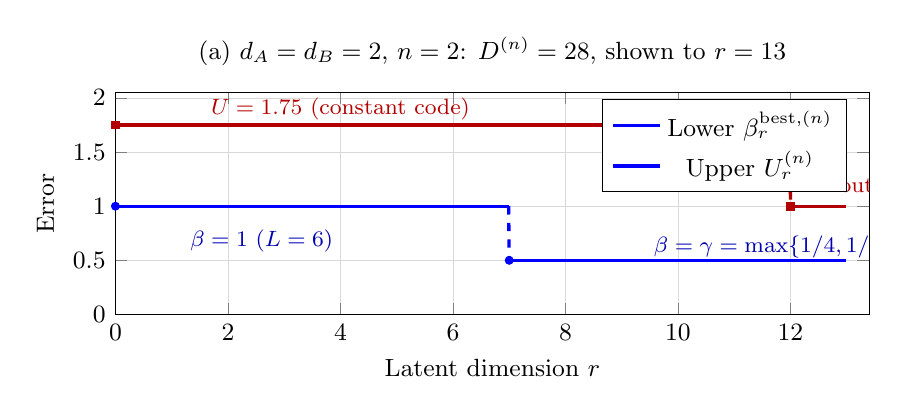
\begin{tikzpicture}
\begin{axis}[
    width=0.92\linewidth, height=4.4cm,
    xlabel={Latent dimension $r$}, ylabel={Error},
    xmin=0, xmax=13.4, ymin=0, ymax=2.05,
    xtick={0,2,4,6,8,10,12}, ytick={0,0.5,1,1.5,2},
    grid=both, grid style={line width=.1pt, draw=gray!30},
    legend pos=north east, legend style={font=\small},
    tick label style={font=\small}, label style={font=\small},
    title={(a) $d_A=d_B=2$, $n=2$: $D^{(n)}=28$, shown to $r=13$},
    title style={font=\small}
]
\addplot[blue, very thick] coordinates {(0,1) (6.99,1)};
\addplot[blue, very thick] coordinates {(7,0.5) (12.99,0.5)};
\addplot[blue, very thick, dashed] coordinates {(6.99,1) (7,0.5)};
\addplot[blue, only marks, mark=*, mark size=1.4pt] coordinates {(0,1) (7,0.5)};
\addplot[red!70!black, very thick] coordinates {(0,1.75) (11.99,1.75)};
\addplot[red!70!black, very thick] coordinates {(12,1) (12.99,1)};
\addplot[red!70!black, very thick, dashed] coordinates {(11.99,1.75) (12,1)};
\addplot[red!70!black, only marks, mark=square*, mark size=1.4pt] coordinates {(0,1.75) (12,1)};
\node at (axis cs:9.4,0.62) [anchor=west, font=\footnotesize, blue!70!black] {$\beta=\gamma=\max\{1/4,1/2\}=1/2$};
\node at (axis cs:4.0,1.9) [font=\footnotesize, red!70!black] {$U=1.75$ (constant code)};
\node at (axis cs:12.7,1.18) [anchor=west, font=\footnotesize, red!70!black] {output pinching $r\ge12$};
\node at (axis cs:2.6,0.68) [font=\footnotesize, blue!70!black] {$\beta=1$ ($L=6$)};
\legend{Lower $\beta_r^{\mathrm{best},(n)}$, Upper $U_r^{(n)}$}
\end{axis}
\end{tikzpicture}

\medskip
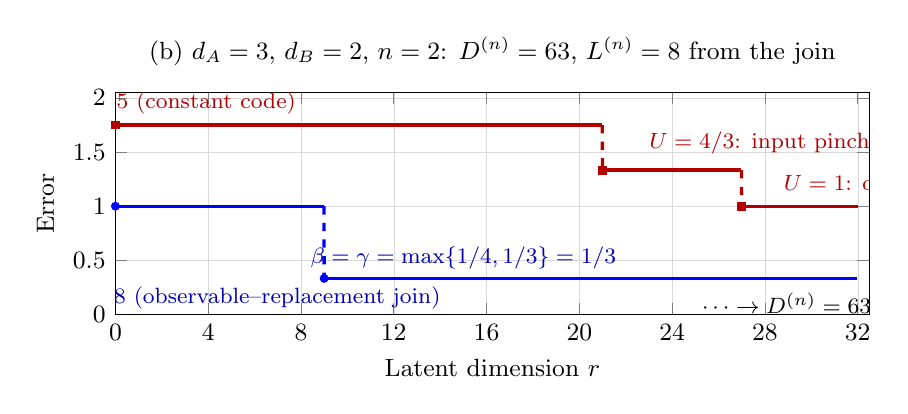
\begin{tikzpicture}
\begin{axis}[
    width=0.92\linewidth, height=4.4cm,
    xlabel={Latent dimension $r$}, ylabel={Error},
    xmin=0, xmax=32.5, ymin=0, ymax=2.05,
    xtick={0,4,8,12,16,20,24,28,32}, ytick={0,0.5,1,1.5,2},
    grid=both, grid style={line width=.1pt, draw=gray!30},
    tick label style={font=\small}, label style={font=\small},
    title={(b) $d_A=3$, $d_B=2$, $n=2$: $D^{(n)}=63$, $L^{(n)}=8$ from the join},
    title style={font=\small}
]
\addplot[blue, very thick] coordinates {(0,1) (8.99,1)};
\addplot[blue, very thick] coordinates {(9,0.333) (31.99,0.333)};
\addplot[blue, very thick, dashed] coordinates {(8.99,1) (9,0.333)};
\addplot[blue, only marks, mark=*, mark size=1.4pt] coordinates {(0,1) (9,0.333)};
\addplot[red!70!black, very thick] coordinates {(0,1.75) (20.99,1.75)};
\addplot[red!70!black, very thick] coordinates {(21,1.333) (26.99,1.333)};
\addplot[red!70!black, very thick] coordinates {(27,1) (32,1)};
\addplot[red!70!black, very thick, dashed] coordinates {(20.99,1.75) (21,1.333)};
\addplot[red!70!black, very thick, dashed] coordinates {(26.99,1.333) (27,1)};
\addplot[red!70!black, only marks, mark=square*, mark size=1.4pt] coordinates {(0,1.75) (21,1.333) (27,1)};
\node at (axis cs:3.2,0.15) [font=\footnotesize, blue!70!black] {$\beta=1$ up to $L=8$ (observable--replacement join)};
\node at (axis cs:15,0.52) [font=\footnotesize, blue!70!black] {$\beta=\gamma=\max\{1/4,1/3\}=1/3$};
\node at (axis cs:22.6,1.58) [anchor=west, font=\footnotesize, red!70!black] {$U=4/3$: input pinching $k_{\mathrm{in}}=3$, $r\ge21$};
\node at (axis cs:28.4,1.2) [anchor=west, font=\footnotesize, red!70!black] {$U=1$: output pinching $r\ge27$};
\node at (axis cs:2.2,1.95) [font=\footnotesize, red!70!black] {$U=1.75$ (constant code)};
\node at (axis cs:33.0,0.1) [anchor=east, font=\footnotesize] {$\cdots\to D^{(n)}=63$};
\end{axis}
\end{tikzpicture}

\medskip
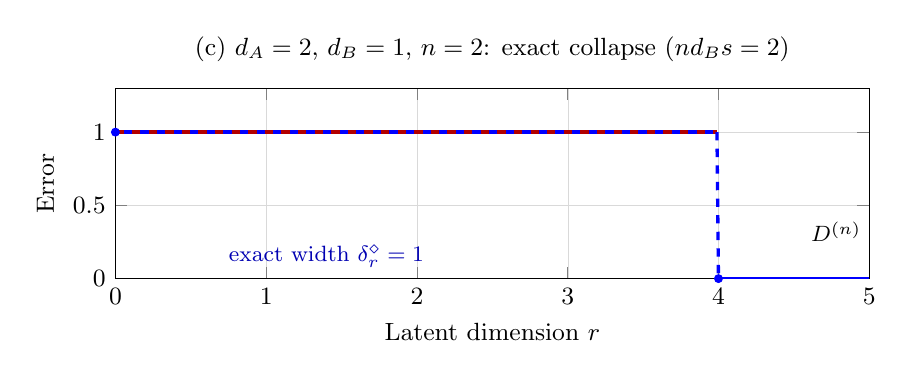
\begin{tikzpicture}
\begin{axis}[
    width=0.92\linewidth, height=4.0cm,
    xlabel={Latent dimension $r$}, ylabel={Error},
    xmin=0, xmax=5, ymin=0, ymax=1.3,
    xtick={0,1,2,3,4,5}, ytick={0,0.5,1},
    grid=both, grid style={line width=.1pt, draw=gray!30},
    tick label style={font=\small}, label style={font=\small},
    title={(c) $d_A=2$, $d_B=1$, $n=2$: exact collapse ($nd_Bs=2$)},
    title style={font=\small}
]
\addplot[blue, very thick] coordinates {(0,1) (3.99,1)};
\addplot[red!70!black, very thick, dashed] coordinates {(0,1) (3.99,1)};
\addplot[blue, very thick, dashed] coordinates {(3.99,1) (4,0)};
\addplot[blue, very thick] coordinates {(4,0) (5,0)};
\addplot[blue, only marks, mark=*, mark size=1.4pt] coordinates {(0,1) (4,0)};
\node at (axis cs:1.4,0.15) [font=\footnotesize, blue!70!black] {exact width $\delta_r^{\diamond}=1$};
\node at (axis cs:4.55,0.32) [anchor=west, font=\footnotesize] {$D^{(n)}=4$};
\end{axis}
\end{tikzpicture}
\caption{Certified lower and upper envelopes of the instrument compression width. (a) The worked example $d_A=d_B=2$, $n=2$ (Example~\ref{ex:222}): $\beta_r^{\mathrm{best},(n)}=1$ for $0\le r\le6$, $\gamma=\max\{\rho_n,1/d_A\}=\max\{1/4,1/2\}=1/2$ for $7\le r<28$, $0$ at $r\ge28$; the upper envelope on the plotted range is $R_{\mathrm{inst}}=2(1-1/8)=1.75$ for the constant code on $0\le r<12$ and $1$ from balanced two-sector output pinching for $12\le r\le13$ ($Q_2(2)=2$, $r_{\mathrm{out}}=12$); the convex-projection bound exceeds $1.75$ on the whole plotted range ($56/29$ at $r=0$, $34/18$ at $r=11$), and input pinching enters only at $r_{\mathrm{in}}=14$, outside the range. (b) $d_A=3$, $d_B=2$, $n=2$: the one-sphere dimension $L^{(n)}=8$ comes from the observable--replacement join (it exceeds both $L_{\mathrm{rep}}=6$ and $L_{\mathrm{obs}}=7$); the upper envelope steps down $1.75\to4/3\to1$ at $r=21$ (three-block input pinching, $Q_3(3)=3$, $r_{\mathrm{in}}=21$) and $r=27$ (two-block output pinching, $r_{\mathrm{out}}=27$), and the intermediate lower bound is $\gamma=1/3$. (c) The exact collapse for $d_A=2$, $d_B=1$, $n=2$ (Theorem~\ref{thm:collapse}): both envelopes equal the exact width, which is the step function $1$ below $D^{(n)}=4$ and $0$ from $D^{(n)}$ on. In panels (a) and (b), filled circles mark the lower envelope and filled squares the upper envelope; in (c) the two envelopes coincide with the exact width, and dashed segments mark the jumps.}
\label{fig:envelope}
\end{figure}

\begin{table}[t]
\centering
\small
\setlength{\tabcolsep}{4pt}
\begin{tabular}{p{3.4cm}p{3.0cm}p{3.0cm}p{3.4cm}}
\toprule
Quantity & Channel $n=1$ & Instrument $n\ge1$ & Origin \\
\midrule
Affine dimension & $d_A^2(d_B^2-1)$ & $d_A^2(nd_B^2-1)$ & $nd_A^2d_B^2-d_A^2$ via surjectivity of the marginal map $(X_1,\dots,X_n)\mapsto\sum_k\Tr_BX_k=H$, e.g.\ $X_1=H\otimes I_B/d_B$\\
Centred in-radius & $2/d_Bs$ & $2/nd_Bs$ & $\max\{0,\lambda_{\max}(-X)\}\le s\|\vD\|_{\diamond,\mathrm{inst}}/2d_A$, $s=\min\{d_A,d_B\}$\\
Covering radius $R(\mathcal I_*)$ & $2(1-1/d_Bs)$ & $2(1-1/nd_Bs)$ & $\sigma_{EBC_n}\le nd_Bs\,(\rho_E\otimes I_B/d_B\otimes I_{C_n}/n)$ plus $a\le Kb$\\
Replacement sphere & $S^{d_B^2-2}$ & $S^{nd_B^2-2}$ & $X\mapsto X_+/t_X$, orthogonal Jordan supports\\
Full-direction sphere & $S^{d_A^2(d_B^2-1)-1}$ & $S^{D^{(n)}-1}$ & Jordan decomposition plus correction state $\nu=(I_{A_0}-\mu)/(d_A-1)$\\
Diamond diameter & $2$ & $2$ & flagged channels have diamond norm $1$; orthogonal flagged states attain $2$\\
Zero-error threshold & $d_A^2(d_B^2-1)$ & $d_A^2(nd_B^2-1)$ & affine coordinates plus Borsuk--Ulam collision\\
\bottomrule
\end{tabular}
\caption{Channel versus instrument exact geometry. The $1/n$ factor is the uniform trace-budget split among $n$ outcomes at the uniform centre; the same numerical positivity budget $2/(nd_Bs)$ is realised by two distinct witnesses --- an orthogonal-output isometry witness for $d_B>1$, and an effect-transfer witness ($\pm\mathcal F/2$) for $d_B=1$, $n\ge2$ --- which live in different faces of the positive cone. Maximality of the radius uses the eigenvalue $1/(nd_Ad_B)-t's/(2d_A)<0$ for $t'>t$, or $1/(nd_A)-t'/(2d_A)<0$ in the POVM case. The sphere rows are stated in the non-singleton regimes ($d_B>1$ for channels, $nd_B>1$ for instruments); the $n=d_B=1$ singleton is described in Remark~\ref{rem:degenerate}.}
\label{tab:comparison}
\end{table}

\begin{table}[t]
\centering
\small
\setlength{\tabcolsep}{4pt}
\begin{tabular}{ccccccccc}
\toprule
$(d_A,d_B,n)$ & $D^{(n)}$ & $L_{\mathrm{rep}}$ & $L_{\mathrm{obs}}$ & $N_{\mathrm{join}}$ & $L_{\mathrm{join}}$ & $L_{A,B}^{(n)}$ & $\gamma_{A,B}^{(n)}$\\
\midrule
$(2,2,2)$ & $28$ & $6$ & $2$ & $2$ & $3$ & $6$ & $1/2$\\
$(3,2,2)$ & $63$ & $6$ & $7$ & $2$ & $8$ & $8$ & $1/3$\\
$(2,3,1)$ & $32$ & $7$ & $2$ & $1$ & invalid & $7$ & $1/2$\\
$(2,1,2)$ & $4$  & $0$ & $2$ & $0$ & invalid & $2$ & $1$\\
\bottomrule
\end{tabular}
\caption{Certified one-sphere dimensions and intermediate envelope value, with $L_{A,B}^{(n)}=\min\{D^{(n)}-1,\max\{L_{\mathrm{rep}},L_{\mathrm{obs}},L_{\mathrm{join}}\}\}$ and $\gamma_{A,B}^{(n)}=\max\{\rho_n,1/d_A\}$. For $(2,1,2)$ one has $nd_Bs=2$ and the collapse of Theorem~\ref{thm:collapse} applies: $\beta_r^{\mathrm{best}}=1$ throughout $r<D$.}
\label{tab:thresholds}
\end{table}

\section{Conclusion}
\label{sec:conclusion}

The exact results of this paper are the affine dimension, the centred in-radius and its global optimality, the covering radius and the diameter, the constant-code width, the zero-error threshold, the replacement profile, and the collapse case, collected in Table~\ref{tab:summary}. The structural fact behind this exactness is the concave--convex duality of the uniform instrument (Theorem~\ref{thm:global-inradius} and Remark~\ref{rem:duality}): the same object is optimal both as the centre of the largest contained ball and as the centre of the smallest covering ball. The intermediate widths, by contrast, are certified rather than exact: the lower envelope combines the two mechanisms of Remark~\ref{rem:gamma-mechanisms}, the upper envelope is attained by explicit constructions, and the bracket between them remains open in general.

The results specialise consistently. For $n=1$ they recover the channel-level theorems of the companion paper~\cite{CompanionChannels}; for $d_B=1$ they govern finite-outcome measurements; and for $d_A=1$ the subcritical widths are exact. The $1/n$ suppression of the centred radius against the $n$-fold growth of the affine dimension (Corollary~\ref{cor:scaling}) quantifies the cost of recording outcomes, and the threshold of Theorem~\ref{thm:collapse} identifies the cases in which the envelopes close.

The following problems remain open: (i) determine the intermediate widths $\delta_{r,\mathrm{inst}}^{\diamond}(A,B)$ for $L_{A,B}^{(n)}<r<D_{A,B}^{(n)}$, or improve either envelope; (ii) determine the largest index $r$ with $\alpha_r(\Inst_n(A,B))=1$; (iii) resolve the boundary cases $c=d_B^2$ and $c=d_A^2d_B^2$ of the scaling trichotomy of Corollary~\ref{cor:scaling}; (iv) determine whether the uniform instrument is the unique optimal centre for the in-radius and for the covering radius.

\section*{Acknowledgements}
The author thanks the anonymous referees for helpful comments.

\appendix

\section{Finite-program evaluation: background}
\label{app:no-programming}

This appendix records, for completeness and motivation, the no-programming obstruction for unitary channels. It is logically independent of the instrument geometry developed above: the main theorems concern \emph{representational} dimension, whereas this appendix concerns \emph{programmable evaluation} with a fixed processor.

\begin{definition}[Exact finite-program evaluator]
Let $E$ and $B$ be finite-dimensional. An exact finite-program evaluator consists of a finite-dimensional program system $M$, a completely positive trace-preserving (CPTP) processor $\Gamma:\Lin(M\otimes E)\to\Lin(B)$, and a program state $\pi_\Phi\in\Sstate(M)$ for every channel $\Phi\in\Chan(E,B)$, such that
\[
\Gamma(\pi_\Phi\otimes\rho)=\Phi(\rho)
\]
for every input state $\rho$ on $E$. By linearity the same identity holds for every input operator.
\end{definition}

\begin{theorem}[No finite exact evaluator for unitary channels]
\label{thm:no-programming}
Let $\dim E>1$. No finite-dimensional program system and fixed CPTP processor $\Gamma:\Lin(M\otimes E)\to\Lin(E)$ can exactly evaluate every unitary channel on $E$.
\end{theorem}

\begin{proof}
For pure program states, the no-programming theorem~\cite{NielsenChuang1997} shows that distinct unitary channels require orthogonal programs. It remains to pass from pure to mixed programs. Suppose
\[
\pi_U=\sum_jq_j|p_j\rangle\langle p_j|,\qquad q_j>0,
\]
is a spectral decomposition of a program that evaluates the unitary channel $\mathcal U_U$. For every pure input $|\psi\rangle$, linearity gives
\[
U|\psi\rangle\langle\psi|U^\dagger
=\sum_jq_j\,\Gamma\big(|p_j\rangle\langle p_j|\otimes|\psi\rangle\langle\psi|\big).
\]
Because $\Gamma$ is CPTP, each summand $\sigma_{j,\psi}$ is a density operator. The right-hand side is a convex decomposition of a pure state, and pure states are extreme points of the state space, so each positive-weight summand equals the same pure output: $\sigma_{j,\psi}=U|\psi\rangle\langle\psi|U^\dagger$ for all $j$ and all pure $|\psi\rangle$. Fixing $j$, the map $\Lambda_j(X)=\Gamma(|p_j\rangle\langle p_j|\otimes X)$ is a channel agreeing with $\mathcal U_U$ on every rank-one projector; rank-one projectors span $\Herm(E)$ over $\mathbb R$, and complex linearity extends the equality to all of $\Lin(E)$. Hence every pure vector in the support of $\pi_U$ programs $\mathcal U_U$ exactly.

Applying the same argument to programs of two distinct unitary channels, the pure-state no-programming theorem makes every positive-weight eigenvector of the first program orthogonal to every positive-weight eigenvector of the second. Those eigenvectors span their respective supports, so $\supp\pi_U\perp\supp\pi_V$. A finite-dimensional program space cannot contain infinitely many mutually orthogonal nonzero supports, while $\dim E>1$ gives infinitely many distinct unitary channels. This proves the claim.
\end{proof}

\begin{corollary}[Unequal output systems]
\label{cor:unequal}
Let $\dim E>1$ and $\dim B\ge\dim E$. There is no finite-dimensional exact evaluator for all channels $E\to B$.
\end{corollary}

\begin{proof}
Choose an isometry $V:E\to B$, let $\iota(\rho)=V\rho V^\dagger$, fix a state $\omega$ on $E$, and define the recovery channel
\[
\mathcal R(\sigma)=V^\dagger\sigma V+\Tr[(I_B-VV^\dagger)\sigma]\,\omega,
\]
which is CPTP and satisfies $\mathcal R\circ\iota=\id_E$. An evaluator for all channels $E\to B$ would in particular evaluate every channel $\iota\circ\mathcal U_U$ for the fixed embedding $\iota$; postcomposing its processor with $\mathcal R$ would then give an exact finite evaluator for all unitary channels on $E$, contradicting Theorem~\ref{thm:no-programming}.
\end{proof}

\begin{corollary}[Vanishing error requires unbounded program dimension]
\label{cor:divergence}
Fix a system $E$ with $\dim E>1$. For each $j$, let $M_j$ be a program system of dimension $m_j$ and let $\Gamma_j:\Lin(M_j\otimes E)\to\Lin(E)$ be a CPTP processor. Write $\Gamma_{j,\pi}(X)=\Gamma_j(\pi\otimes X)$ and suppose
\[
\sup_{U\in\mathrm U(E)}\min_{\pi\in\Sstate(M_j)}
\|\Gamma_{j,\pi}-\mathcal U_U\|_\diamond
\le\varepsilon_j,\qquad\varepsilon_j\longrightarrow0.
\]
Then $m_j\to\infty$.
\end{corollary}

\begin{proof}
Suppose otherwise. Passing to a subsequence, assume $m_j\le m_{\max}$ for every $j$. Let $M\simeq\mathbb C^{m_{\max}}$ and choose isometries $W_j:M_j\to M$. Put $P_j=W_jW_j^\dagger$, fix $\tau_j\in\Sstate(M_j)$, and define
\[
\Lambda_j(\eta)=W_j^\dagger P_j\eta P_jW_j+\Tr[(I_M-P_j)\eta]\,\tau_j,
\]
a CPTP map $\Lin(M)\to\Lin(M_j)$: the first term is the compression onto the $P_j$-corner followed by the isometry $W_j^\dagger$, and the second is a measure-and-prepare channel on the orthocomplement (the two trace contributions add up to $\Tr\eta$). In particular $\Lambda_j(W_j\pi W_j^\dagger)=\pi$ for $\pi\in\Sstate(M_j)$. The extended processors $\widetilde\Gamma_j=\Gamma_j\circ(\Lambda_j\otimes\id_E):\Lin(M\otimes E)\to\Lin(E)$ are CPTP and preserve every originally programmed channel. The set of CPTP maps on the fixed spaces $M\otimes E\to E$ is compact, so, passing to a further subsequence \emph{chosen independently of the target unitary}, $\widetilde\Gamma_j\to\Gamma$ in diamond norm. Now fix a unitary $U$. For each $j$ choose $\pi'_j(U)\in\Sstate(M_j)$ with approximation error at most $\varepsilon_j$ (such a minimiser exists by compactness of $\Sstate(M_j)$ and continuity of the induced channel), and embed it as $\pi_j(U)=W_j\pi'_j(U)W_j^\dagger\in\Sstate(M)$. By compactness of $\Sstate(M)$ there is a $U$-dependent subsubsequence with $\pi_j(U)\to\pi_U$; along it the processors still converge to the same $\Gamma$. Continuity of the evaluation map in both processor and program state gives $\Gamma(\pi_U\otimes\cdot)=\mathcal U_U$. Since $U$ was arbitrary, the single limiting processor $\Gamma$ exactly evaluates every unitary channel, contradicting Theorem~\ref{thm:no-programming}. Hence no bounded subsequence of $(m_j)$ exists, and, $(m_j)$ being integer-valued, $m_j\to\infty$.
\end{proof}

\begin{remark}[Scope of the no-programming obstruction]
\label{rem:scope}
The result forbids a scheme that is simultaneously exact, deterministic, universal over the unitary promise class, and finite-dimensional. It does not forbid approximate, probabilistic, restricted-family, infinite-dimensional, or unbounded-register schemes, nor schemes with an externally supplied classical description. A finite classical program register is still a finite-dimensional program and is not exempt. Storing a Choi operator as a mathematical state is also distinct from evaluating the represented channel with one fixed CPTP processor. The optimal asymptotic program cost of approximate universal unitary programming is determined in~\cite{YangRennerChiribella2020}, and quantitative program-dimension lower bounds in the approximate case are obtained in~\cite{KubickiPalazuelosPerezGarcia2019}; the compactness corollary above records the qualitative divergence consequence needed for motivation. Complementary quantitative statements --- the positive finite-programming floor, program-state separation, and the packing lower bounds --- are developed in the companion paper~\cite{CompanionChannels}.
\end{remark}

\begin{thebibliography}{99}

\bibitem{Choi1975}
M.-D. Choi, \emph{Completely positive linear maps on complex matrices}, Linear Algebra Appl. \textbf{10}, 285--290 (1975).

\bibitem{CompanionChannels}
Anonymous, \emph{Exact diamond balls, antipodal widths, and query-uniform compression bounds for quantum channels}, companion manuscript.

\bibitem{Jamiolkowski1972}
A.~Jamio{\l}kowski, \emph{Linear transformations which preserve trace and positive semidefiniteness of operators}, Rep. Math. Phys. \textbf{3}, 275--278 (1972).

\bibitem{KubickiPalazuelosPerezGarcia2019}
A.~M. Kubicki, C. Palazuelos, and D. P\'erez-Garc\'ia, \emph{Resource quantification for the no-programing theorem}, Phys. Rev. Lett. \textbf{122}, 080505 (2019).

\bibitem{DaviesLewis1970}
E.~B. Davies and J.~T. Lewis, \emph{An operational approach to quantum probability}, Commun. Math. Phys. \textbf{17}, 239--260 (1970).

\bibitem{AharonovKitaevNisan1998}
D. Aharonov, A. Kitaev, and N. Nisan, \emph{Quantum circuits with mixed states}, in Proceedings of the Thirtieth Annual ACM Symposium on Theory of Computing (STOC 1998), ACM, New York, 1998, pp.~20--30.

\bibitem{Ozawa1984}
M. Ozawa, \emph{Quantum measuring processes of continuous observables}, J. Math. Phys. \textbf{25}, 79--87 (1984).

\bibitem{Pinkus1985}
A. Pinkus, \emph{$n$-Widths in Approximation Theory}, Ergebnisse der Mathematik und ihrer Grenzgebiete \textbf{7}, Springer, Berlin, 1985.

\bibitem{ChiribellaEtAl2009Instruments}
G. Chiribella, G.~M. D'Ariano, and P. Perinotti, \emph{Realization schemes for quantum instruments}, J. Math. Phys. \textbf{50}, 042101 (2009).

\bibitem{ChiribellaEtAl2008Combs}
G. Chiribella, G.~M. D'Ariano, and P. Perinotti, \emph{Quantum circuit architecture}, Phys. Rev. Lett. \textbf{101}, 060401 (2008).

\bibitem{Helstrom1976}
C.~W. Helstrom, \emph{Quantum Detection and Estimation Theory}, Mathematics in Science and Engineering \textbf{123}, Academic Press, New York, 1976.

\bibitem{Watrous2018}
J. Watrous, \emph{The Theory of Quantum Information}, Cambridge University Press (2018).

\bibitem{NielsenChuang1997}
M.~A. Nielsen and I.~L. Chuang, \emph{Programmable quantum gate arrays}, Phys. Rev. Lett. \textbf{79}, 321--324 (1997).

\bibitem{YangRennerChiribella2020}
Y. Yang, R. Renner, and G. Chiribella, \emph{Optimal universal programming of unitary gates}, Phys. Rev. Lett. \textbf{125}, 210501 (2020).

\bibitem{Matousek2003}
J. Matou{\v{s}}ek, \emph{Using the Borsuk--Ulam Theorem}, Springer (2003).

\bibitem{Barvinok2002}
A. Barvinok, \emph{A Course in Convexity}, Graduate Studies in Mathematics \textbf{54}, AMS (2002).

\end{thebibliography}

\end{document}
